\documentclass[11pt]{article}

\usepackage[paperheight=23 cm, paperwidth=17 cm, top=2 cm, bottom=2 cm, left=2.5 cm, right=1.5 cm]{geometry}
\usepackage[spanish,mexico]{babel}
\usepackage{amsmath} % Some math functions
\usepackage{amsfonts} % Some math functions
\usepackage{subcaption} % Subfigures
\usepackage[utf8]{inputenc}
\usepackage{lscape} % Landscape mode
\usepackage[nottoc]{tocbibind} % Include bibliography in TOC
\usepackage{url}
%\usepackage{array}
%\usepackage[toc,page]{appendix}

\usepackage[letter,cam,center]{crop} % Crop marks
\usepackage[labelfont=bf]{caption}

\usepackage{graphicx} % OS X

%\usepackage[pdftex]{graphicx} % Windows
%\usepackage{epstopdf} % Windows

%\renewcommand{\baselinestretch}{1.6} %double-spacing

\let\EndItemize\enditemize
\def\enditemize{\EndItemize\bigskip} %space after itemize

\numberwithin{equation}{section} %equation numbers
%DIF PREAMBLE EXTENSION ADDED BY LATEXDIFF
%DIF UNDERLINE PREAMBLE %DIF PREAMBLE
\RequirePackage[normalem]{ulem} %DIF PREAMBLE
\RequirePackage{color}\definecolor{RED}{rgb}{1,0,0}\definecolor{BLUE}{rgb}{0,0,1} %DIF PREAMBLE
\providecommand{\DIFadd}[1]{{\protect\color{blue}\uwave{#1}}} %DIF PREAMBLE
\providecommand{\DIFdel}[1]{{\protect\color{red}\sout{#1}}}                      %DIF PREAMBLE
%DIF SAFE PREAMBLE %DIF PREAMBLE
\providecommand{\DIFaddbegin}{} %DIF PREAMBLE
\providecommand{\DIFaddend}{} %DIF PREAMBLE
\providecommand{\DIFdelbegin}{} %DIF PREAMBLE
\providecommand{\DIFdelend}{} %DIF PREAMBLE
%DIF FLOATSAFE PREAMBLE %DIF PREAMBLE
\providecommand{\DIFaddFL}[1]{\DIFadd{#1}} %DIF PREAMBLE
\providecommand{\DIFdelFL}[1]{\DIFdel{#1}} %DIF PREAMBLE
\providecommand{\DIFaddbeginFL}{} %DIF PREAMBLE
\providecommand{\DIFaddendFL}{} %DIF PREAMBLE
\providecommand{\DIFdelbeginFL}{} %DIF PREAMBLE
\providecommand{\DIFdelendFL}{} %DIF PREAMBLE
%DIF END PREAMBLE EXTENSION ADDED BY LATEXDIFF

\begin{document}

\thispagestyle{empty}
\tableofcontents
\clearpage

\setcounter{page}{1}

\section{Introducción}

Los mercados de valores permiten el intercambio de activos con relativa facilidad. La mayoría de los estudios del mercado tratan de explicar su comportamiento a través de procesos autorregresivos con el objetivo de establecer la relación del valor actual de una serie de tiempo con los valores anteriores; sin embargo, la mayoría de estos estudios ignoran el mecanismo básico detrás de estos mercados: la lógica racional de oferta y demanda entre compradores y vendedores.\\

Los mercados se pueden clasificar en dos tipos:
\begin{itemize}
  \item Regidos por formadores de mercado (Quote-driven market)
  \item Regidos por órdenes (Order-driven market)
\end{itemize}

En los mercados regidos por formadores de mercado, éstos centralizan las órdenes proveyendo liquidez al fijar una postura de compra y una de venta; un ejemplo de esto es el especialista en el NYSE, el cual es el punto de contacto entre compradores y vendedores. El especialista tiene como misión mantener la continuidad del mercado, mantener a los inversionistas informados, comprometer capital cuando es necesario y asegurar equidad de oportunidades entre todos los clientes \cite{nyse}. En los mercados regidos por órdenes, las posturas de todos los participantes se agregan en lo que se conoce como el libro de posturas. Los inversionistas ingresan lo que se conoce como posturas limitadas (con un precio limite de compra o venta según corresponda) en el libro de posturas, por lo que éste también se conoce como libro de posturas limitado. Los mercados regidos por órdenes tienen la ventaja de dar transparencia a todos los participantes, ya que éstos conocen las características de cada una de las posturas. De igual forma, existen algunos mercados híbridos donde los formadores de mercado interactúan en el libro de posturas; la Bolsa Mexicana de Valores y NASDAQ son algunos ejemplos.\\

La microestructura del mercado se define como el estudio del proceso y los resultados del intercambio de activos bajo un conjunto especifico de reglas \cite{1995market}. El estudio de la microestructura del mercado es de utilidad ya que permite identificar patrones dentro del mismo. Estos patrones pueden ser utilizados para la predicción de los movimientos del mercado y para la identificación de comportamientos fraudulentos entre los participantes del mercado como se ha hecho en otros trabajos \cite{manipulation}. Esta información es de gran interés para los reguladores, ya que permite identificar casos de manipulación de precios.
\\

Con el objetivo de estudiar el comportamiento de la Bolsa Mexicana de Valores, se obtuvo una base de datos con todas las posturas del libro de órdenes en un periodo determinado. El trabajo se divide en dos partes; en la primera, se describirá la base datos sujeta al estudio y se explicará la forma en que se reconstruyó el libro de posturas para llevar a cabo el análisis. Los resultados obtenidos tras la reconstrucción se compararán con los estudios de otros mercados similares. En la segunda, se describirá un modelo del libro de posturas y un método basado en la transformación inversa de Laplace para llevar a cabo la predicción del movimiento en el precio de una emisora. Se considera que esta es la primera vez que se realiza un análisis como éste con los datos de la BMV.

\clearpage

\section{Descripción de la Base de Datos}
La Bolsa Mexicana de Valores proporcionó para este trabajo una base de datos con las posturas en todas las emisoras entre el 16 de noviembre de 2010 y el 18 de febrero de 2011. La base de datos se compone de dos tablas:

\begin{itemize}
  \item Registro de Posturas
  \item Posturas Iniciales
\end{itemize}

La tabla de registro tiene 25,491,702 renglones; mientras que la tabla de posturas iniciales tiene 275,005. En el registro se encuentran todas las posturas que se reciben a lo largo del día, mientras que en la tabla de posturas iniciales, se almacenan todas la posturas que se recibieron en el registro y siguen vigentes al terminar el día. La tabla de posturas iniciales se utiliza al empezar cada día para cargar las posturas antes mencionadas. Las tablas tienen los siguientes campos:\\

\noindent
\begin{tabbing}
\textbf{id} \hspace{3cm} \= Número de identificación \hspace{1cm} \= \\
\\
\textbf{folio} \> Número asignado por la BMV a la postura\\
Según el reglamento de la BMV; las órdenes que, en su caso, tengan modificaciones,\\
perderán el folio de recepción que en un inicio les haya correspondido y se les asignará\\
uno nuevo. No perderán su folio aquellas órdenes que sean modificadas únicamente\\
para disminuir su volumen.\\
\\
\textbf{fecha\_vig/vigencia} \> Fecha de vigencia de la postura \\
\\
\textbf{casabolsa} \> Casa de Bolsa\\
\\
\textbf{tipo\_mov} \> Tipo de Movimiento\\
\underline{Posibles Valores} \\
CO \> Compra\\
VE \> Venta\\
MO \> Modificación\\
CA \> Cancelación\\
AH \> Reconocimiento de Hecho\\
MH \> Modificación de Hecho\\
CH \> Cancelación de Hecho\\
\\
\textbf{tipo\_op} \> Tipo de Operación\\
\underline{Posibles Valores} \\
CO \> Contado\\
PI \> Pico\\
Son operaciones que implican la compra/venta de una cantidad de acciones inferior\\
a un lote (para la mayoría de la emisoras son 100 acciones).\\
HC \> Operación a Precio de Cierre\\
DC \> Operaciones al Precio de Cierre Modalidad Después del Cierre\\
OR \> Operaciones de Registro\\
OP \> Oferta Pública\\
SR \> Suscripción Recíproca\\
SA \> Sobre Asignación\\
\\
\textbf{tipo\_ord} \> Tipo de Orden\\
\underline{Posibles Valores} \\
LP \> Limitada\\
MC \> Mercado\\
MA \> Mejor Postura Limitada Activa\\
Aquella que sigue el mejor precio límite visible en su mismo sentido y su precio \\
buscará cerrar posturas en sentido contrario que se ubiquen dentro de su precio\\
de protección.\\
MP \> Mejor Postura Limitada Pasiva\\
Aquella que sigue el mejor precio límite visible en su mismo sentido. Aún y cuando\\
existan posturas en sentido contrario dentro de su precio de protección la postura\\
no buscará cerrarlas.\\
VO \> Postura Limitada con Volumen Oculto\\
LO \> Mejor Postura Limitada Activa con Volumen Oculto\\
HC \> Operación a Precio de Cierre\\
DC \> Operaciones al Precio de Cierre Modalidad Después del Cierre\\
PQ \> Paquete \\
\\
\textbf{tipo\_val} \> Tipo de Valor\\
\\
\textbf{emisora} \> Emisora\\
\\
\textbf{serie} \> Serie\\
\\
\textbf{precio} \> Precio\\
\\
\textbf{volumen} \> Volumen\\
\\
La tabla de posturas iniciales utiliza además estos campos:\\
\\
\textbf{fecha} \> Fecha\\
Este campo se utiliza para distinguir las órdenes que están activas al principio del\\
día, actualiza las posiciones activas para inicializar el libro de órdenes.\\
\\
\textbf{orig\_timestamp} \> Fecha original de la postura expresada como la cantidad de\\
\> milésimas de segundo transcurridas desde la medianoche del\\
\>1 de enero de 1970\\
\\
La tabla de registro utiliza estos campos:\\
\\
\textbf{timestamp} \> Fecha de la postura expresada como la cantidad de milésimas\\
\> de segundo transcurridas desde la medianoche del 1 de enero\\
\>de 1970\\
\\
\textbf{folio\_anterior} \> Folio Anterior\\
Se utiliza para localizar el folio de una postura que se va a modificar o cancelar.\\
\\
\textbf{fecha\_folio\_ant} \> Fecha de Folio Anterior\\
\end{tabbing}

\begin{landscape}

\begin{table}[htbp]\scriptsize
\centering
\caption{Posturas Iniciales}
\setlength\tabcolsep{1.5pt}
\begin{tabular}{rrrrrrrrrrrrrr}
\textbf{ id}    & \textbf{fecha} & \textbf{orig\_timestamp} & \textbf{folio} & \textbf{fecha\_vig} & \textbf{tipo\_mov} & \textbf{casabolsa} & \textbf{tipo\_op} & \textbf{tipo\_ord} & \textbf{tipo\_val} & \textbf{emisora} & \textbf{serie} & \textbf{precio} & \textbf{volumen} \\
247 & 24/11/2010 & 1290011934040 & 318480 & 10/12/2010 & CO    & 1277  & CO    & LP    & 1     & LAB   & B     & 25.95 & 2700 \\
292 & 23/11/2010 & 1290189919100 & 368726 & 26/11/2010 & VE    & 1392  & CO    & LP    & 1     & CHDRAUI & B     & 39.8  & 100 \\
519 & 23/12/2010 & 1292863358080 & 242642 & 24/12/2010 & VE    & 1277  & CO    & LP    & 1     & TELMEX & L     & 10.18 & 25000 \\
651 & 27/01/2011 & 1295881813280 & 93317 & 28/01/2011 & VE    & 1664  & CO    & LP    & 1     & ASUR  & B     & 72    & 100 \\
848 & 15/02/2011 & 1295539042060 & 268023 & 18/02/2011 & CO    & 1392  & CO    & LP    & 1     & INCARSO & B-1   & 12.01 & 1000 \\
\ldots & \ldots & \ldots & \ldots & \ldots & \ldots & \ldots & \ldots & \ldots & \ldots & \ldots & \ldots & \ldots & \ldots \\
\end{tabular}%
\label{tab:posinicialesl}%
\end{table}%

\begin{table}[htbp]\scriptsize
\centering
\caption{ Registro de Posturas}
\setlength\tabcolsep{1.25pt}
\begin{tabular}{rrrrrrrrrrrrrrr}
\textbf{ id}    & \textbf{timestamp} & \textbf{folio} & \textbf{vigencia} & \textbf{folio\_anterior} & \textbf{fecha\_folio\_ant} & \textbf{tipo\_mov} & \textbf{casa\_bolsa} & \textbf{tipo\_op} & \textbf{tipo\_ord} & \textbf{tipo\_val} & \textbf{emisora} & \textbf{serie} & \textbf{precio} & \textbf{volumen} \\
48 & 1289916001700 & 19    &       & 0     &       & VE    & 1369  & CO    & LP    & 1     & ARA & *     & 39.6  & 800 \\
329 & 1290785630710 & 124082 & 26/11/2010 & 0     &       & CO    & 1369  & CO    & LP    & 1     & AMX   & L     & 35.69 & 12000 \\
519 & 1291907916550 & 16032 &       & 0     &       & AH    & 1305  & CO    & VO    & 1     & GNP & *     & 58.1  & 1100 \\
652 & 1296246310460 & 911020 &       & 0     &       & VE    & 1369  & PI    & MC    & 1     & ASUR  & B     & 64.05 & 76 \\
998 & 1298062094720 & 566388 & 18/02/2011 & 566388 & 18/02/2011 & MO    & 1288  & CO    & MA    & 1     & BIMBO & A     & 97.51 & 300 \\
\ldots & \ldots & \ldots & \ldots & \ldots & \ldots & \ldots & \ldots & \ldots & \ldots & \ldots & \ldots & \ldots & \ldots & \ldots \\
\end{tabular}%
\label{tab:regposturasl}%
\end{table}%

\end{landscape}

\clearpage

\section{Reconstrucción del Libro de Posturas}

Para realizar los diversos análisis fue necesario reconstruir el libro de posturas. El libro de posturas registra todas las posturas para cada una de las emisoras. Por reconstruir, en este trabajo se entiende tomar el registro cronológico de las posturas de compra y venta proporcionado por la BMV, con el fin de determinar el volumen y precio de las posturas activas en cada instante de tiempo, agrupándolas por precio. Uno de los principales retos que se identificaron fueron las modificaciones y cancelaciones. A lo largo del día existen un gran número de modificaciones y cancelaciones; aproximadamente el 11\% de los registros en la base de datos son modificaciones y el 35\% son cancelaciones. Por lo tanto, es indispensable identificar las posturas activas en todo momento. En otros trabajos esto no ha presentado un reto ya que se ha contado con una representación del libro que facilita el análisis. Trabajos anteriores \cite{biais1995,Cont2010,zhao2010} han realizado el análisis con lo que se conoce como las ``puntas''. Las puntas son las mejores posturas de compra y venta en el libro de posturas. El análisis que se realiza en este trabajo es más completo ya que cuenta con la información de todas las posturas en cada instante de tiempo.\\

Otro reto que se identificó fue el de las posturas de tipo VO (Volumen Oculto). La base de datos que se utilizó no cuenta con la información del volumen que se encuentra oculto en este tipo de órdenes. Se optó por ignorar esta información ya que las posturas de tipo VO comprenden sólo el 0.55\% del total, mientras que las de tipo LP (Limitadas), las más comunes, representan el 93.81\%; estas últimas sí cuentan con la información del volumen. Como se muestra más adelante, ignorar las posturas de tipo VO no tuvo un gran impacto ya que los hechos reportados por el algoritmo son similares a los reportados por la BMV. Las operaciones del tipo PI (Picos) representan el 0.61\% de la muestra y de acuerdo al reglamento de la BMV no se incluyen en el libro de posturas, por lo que para el análisis también se ignoraron. Adicionalmente el algoritmo respeta el horario establecido en el reglamento de la bolsa; por lo tanto, antes de las 8:30am no se concreta ningún hecho. En la primera fase, el algoritmo carga las posturas que quedaron abiertas en días anteriores de la tabla de Posturas Iniciales y en la segunda se procesa el registro.\\

El algoritmo se implementó en Java y se desarrolló una interfaz gráfica. Como se puede ver en la Figura \ref{java}, la interfaz permite analizar individualmente cada entrada del registro de una emisora para un día. La interfaz cuenta con 5 ventanas:
\begin{itemize}
  \item Corros de Venta
  \item Corros de Compra
  \item Hechos Reportados por la BMV
  \item Hechos Reportados por el Algoritmo
  \item Registro
\end{itemize}

Con el botón de ``Siguiente'' se van procesando una a una las entradas del registro. En el caso de una postura de compra, se trata de buscar una postura en los corros de venta para perfeccionarla (perfeccionar en este caso se entiende en el sentido utilizado por la BMV, es decir, completar los requisitos para que un acto jurídico tenga plena validez); si no existe, ésta se registra en los corros de compra, los cuales están ordenados de mayor a menor precio. El mismo procedimiento se realiza para las posturas de venta, de tal forma, que la postura que se encuentra en la parte inferior de los corros de venta y la que se encuentra en la parte más alta de los corros de compra se conocen como las puntas. Una función adicional de la interfaz es la cancelación de posturas de compra o de venta. Las posturas se cancelan al seleccionarlas y oprimir el botón correspondiente. Esta función se implementó con el objeto de poder depurar errores en el funcionamiento del algoritmo.\\

Como se mencionó antes, los hechos se registran con la clave AH; éstos se mantienen en la ventana de ``Hechos Registrados por la BMV''. Cuando el algoritmo desarrollado perfecciona un hecho, éste se registra en la ventana de ``Hechos Reportados por el Algoritmo''. Para las cancelaciones y las modificaciones, es necesario localizar el folio correspondiente en los corros de compra o venta para realizar lo que a cada una corresponde. Con el objetivo de poder analizar el registro con mayor rapidez, se implementó el botón de ``Play'', el cual permite avanzar 100 entradas del registro.

\begin{landscape}

\begin{figure}[htbp] \centering
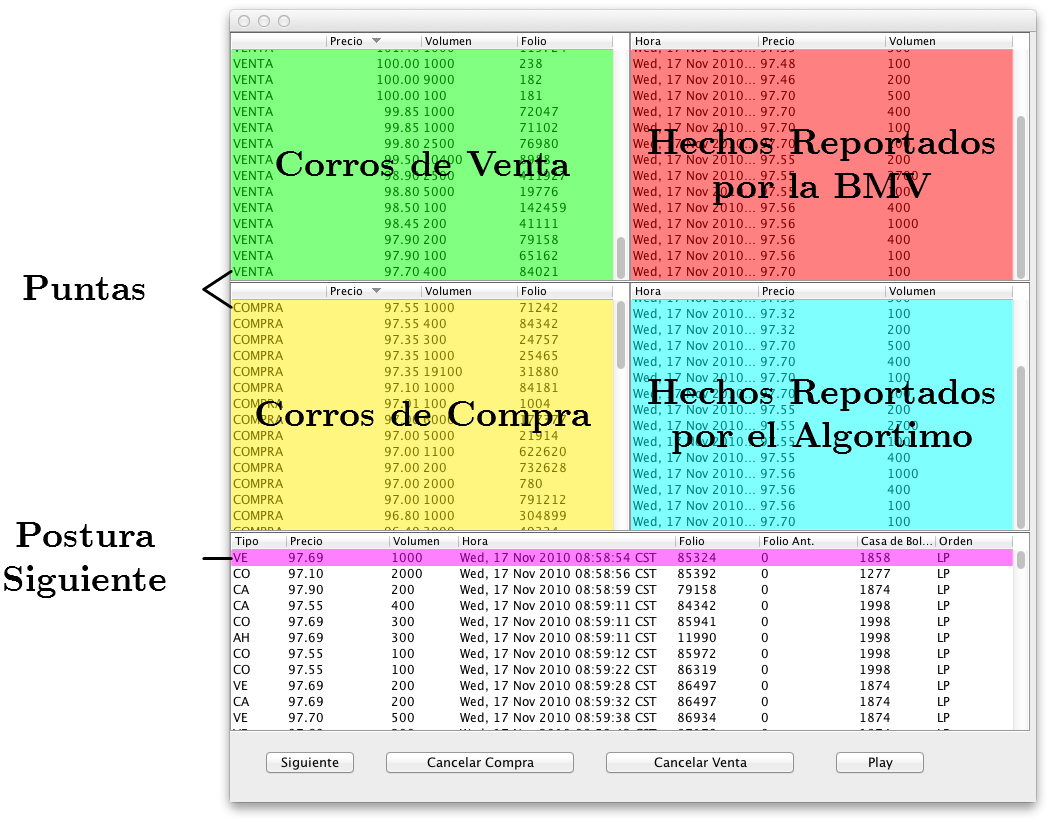
\includegraphics{screenshot.png}
\caption{Captura de pantalla de la Interfaz desarrollada en Java}
\label{java}
\end{figure}

\end{landscape}

Para medir la efectividad del algoritmo se compararon los hechos reportados por la BMV con los hechos arrojados por el algoritmo y se ignoraron acciones de muy baja bursatilidad. Por ejemplo, se analizó la acción de KUO serie B. Ésta tiene en promedio alrededor de 28 posturas diarias en la base de datos comparado con la media de 2,550 posturas diarias para las demás emisoras; y se observó que para la muestra de 68 días, el algoritmo solamente reprodujo el 50.3\% del volumen operado según la BMV. Al realizar un análisis más profundo del volumen operado de esta acción durante el plazo mencionado, se encontró que la baja efectividad del algoritmo se debe a una serie de posturas de volumen oculto que se registraron el 29 de diciembre de 2010. Si se excluye esta fecha, el algoritmo reporta un volumen de 5,607,600 acciones mientras que la BMV reporta 5,972,500, es decir, el algoritmo tiene una efectividad del 93.9\%. Para AMX serie L, la acción con mayor volumen en la BMV con un promedio 44,396 posturas por día, el algoritmo reproduce el 89.7\% de las operaciones.\\


No sólo es importante analizar el volumen operado, sino también la evolución del precio de una acción. Para realizar el análisis de la tendencia del precio, se utilizó el precio promedio ponderado por volumen, VWAP (Volume-weighted average price). Para la acción de KUO el VWAP del 28 de enero de 2011 registrado por la BMV es de 21.72491, el registrado por el algoritmo es de 21.72289. Por ejemplo, el 31 de diciembre de 2010 se encontró una diferencia entre el volumen reportado por la bolsa y el del algoritmo mayor al 50\%; sin embargo, el VWAP de la bolsa y del algoritmo son similares, 20.35595 y 20.27741 respectivamente. En la Figura \ref{kuo1231} y la Figura \ref{kuo0128} se muestra de forma gráfica la evolución del precio de KUO a lo largo de los días mencionados antes.\\

Para el caso de AMX, el 28 de diciembre el algoritmo tuvo solamente un 69.0\% de efectividad para replicar el volumen, sin embargo, el VWAP de la bolsa y el algoritmo difieren en menos de 0.08\%. El 20 de enero de 2011, día de mayor efectividad en términos del volumen, la bolsa reporta un VWAP de 35.28202 mientras que el algoritmo 35.26883. En la Figura \ref{amx0120} y la Figura \ref{amx1228} se encuentran unas gráficas con los precios de AMX a lo largo de esos días. Como se puede notar en la Figura \ref{amx0120}, existen momentos en que los hechos reportados por la BMV y el algoritmo son muy distintos. Por ejemplo, cercano a las 9:30am, el algoritmo registra un hecho a 35.00 mientras que la BMV lo registra a 35.22; esto se debe a las deficiencias que se mencionaron antes en la base de datos. Sin embargo, como se mostró ya el VWAP reportado por ambos es similar.

\begin{figure}[htbp] \centering
\includegraphics[scale=0.75, trim=0 0.5cm 0 1.5cm]{kuo123110.eps}
\caption{Reconstrucción: KUO diciembre 31}
\label{kuo1231}
\end{figure}

\begin{figure}[htbp] \centering
\includegraphics[scale=0.75, trim=0 0.5cm 0 1.5cm]{kuo012811.eps}
\caption{Reconstrucción: KUO enero 28}
\label{kuo0128}
\end{figure}

\begin{figure}[htbp] \centering
\includegraphics[scale=0.75, trim=0 0.5cm 0 1.5cm]{amx012011.eps}
\caption{Reconstrucción: AMX enero 20}
\label{amx0120}
\end{figure}

\begin{figure}[htbp] \centering
\includegraphics[scale=0.75, trim=0 0.5cm 0 1.5cm]{amx122810.eps}
\caption{Reconstrucción: AMX diciembre 28}
\label{amx1228}
\end{figure}

\clearpage

\section{Características Estadísticas del Libro de Posturas}

Los mercados financieros son inherentemente difíciles de analizar; sin embargo, es posible identificar algunos patrones en su comportamiento. Estudios anteriores \cite{Bouchaud2002,zovko2002power,marketsdigest} han identificado patrones para el desempeño de precios, volúmenes y cancelaciones en el libro de posturas. A continuación, se compararán resultados obtenidos en otros mercados con una muestra de acciones de la Bolsa Mexicana de Valores. Para la muestra se eligieron emisoras de alta bursatilidad (AMX), media (BIMBO, COMERCI y GRUMA) y baja (HERDEZ y KUO). Este análisis podría extenderse fácilmente a otras acciones.\\

\subsection{Precios}

Para los precios, se ha identificado que la distribución de sus posturas sigue una ley de potencias \cite{Bouchaud2002}, es decir, que las frecuencias decrecen exponencialmente al aumentar el precio. Es importante mencionar que en \cite{Bouchaud2002} y otros trabajos no se presentan pruebas de hipótesis de esto.\\

Si se define a $b(t)$ como el precio de la mejor postura de compra (``bid'') y $a(t)$ como el precio de la mejor postura de venta (``ask''), el precio de una nueva postura de compra o venta se puede expresar como $b(t)-\Delta$ ó $a(t)+\Delta$ respectivamente, donde la $\Delta$ está expresada en pujas o ticks. Una puja es el importe mínimo en que puede variar el precio unitario de cada título. Cabe mencionar que $\Delta$ puede tomar valores negativos. Si por ejemplo, con $\Delta <0$, se registra una postura con el precio $b(t)-\Delta \geq a(t)$ entonces se concretará un hecho, mientras que si $b(t)-\Delta < a(t)$ entonces el precio $b(t+1)=b(t)-\Delta$. Si se excluyen las posturas donde $\Delta \leq 0$, se puede decir que los precios siguen una distribución definida por la siguiente función de densidad:

\begin{equation}
P\left(\Delta\right) \propto \frac{A}{{\left(\Delta+\lambda\right)}^{\alpha+1}}
\end{equation}

Con el objetivo de analizar si el comportamiento de los precios de la Bolsa Mexicana sigue los patrones antes mencionados, se estimaron los parámetros del modelo utilizando el método de máxima verosimilitud (en la Sección \ref{sec:estim} se realiza un análisis de los estimadores utilizados) para distintas acciones, excluyendo todas las modificaciones, las cuales se podrían en algunos casos considerar como una nueva postura. Otros estudios han encontrado que el parámetro $\alpha$ es ``similar'' entre las distintas emisoras \cite{zovko2002power} de un mercado en particular, sin embargo, como se puede ver en las Tablas \ref{tab:powercompra} y \ref{tab:powerventa}, las acciones de la BMV tienen parámetros distintos. La distribución ajustada es conocida como Lomax o Pareto Tipo II con $\mu=0$. La media de esta distribución está definida cuando $\alpha>1$; en este análisis existen algunas emisoras para las que no se podría definir la media. En otros estudios se destaca que el parámetro $\alpha$ es similar para las posturas de compra y venta de una misma emisora \cite{Bouchaud2002}. En las acciones utilizadas en este trabajo el parámetro es similar en la mayoría de los casos; sin embargo, en el caso de KUO el parámetro $\alpha$ para las posturas de venta es 50\% mayor que el de las de compra.\\

\begin{table}[htbp]
\centering
\caption{Distribución de Precios de las Posturas de Compra}
\renewcommand{\arraystretch}{1.2}
\begin{tabular}{r|r|r|r|r|r|r|}
\cline{2-7}
& $\lambda$ & $\alpha$ & \#posturas & $\Delta>0$ & $D_n$ & $\bar{D}$ \\
\cline{2-7}
\textbf{AMX}   & 7.4441 & 1.7098 & 629,302 & 454,039 & 0.2276 & 0.1562 \\
\textbf{BIMBO} & 14.7809 & 0.8242 & 37,021 & 9,042 & 0.0928 & 0.0375 \\
\textbf{COMERCI}   & 7.6756 & 1.2256 & 20,955 & 4,201 & 0.0754 & 0.0307 \\
\textbf{GRUMA} & 58.6601 & 4.4624 & 49,895 & 27,845 & 0.1172 & 0.0832 \\
\textbf{HERDEZ} & 21.1333 & 2.3332 & 6,811 & 1,773 & 0.1337 & 0.0675 \\
\textbf{KUO}   & 11.3803 & 0.8556 & 495 & 93 & 0.0660 & 0.0360 \\
\cline{2-7}
\end{tabular}%
\label{tab:powercompra}%
\end{table}%

\begin{table}[htbp]
\centering
\caption{Distribución de Precios de las Posturas de Venta}
\renewcommand{\arraystretch}{1.2}
\begin{tabular}{r|r|r|r|r|r|r|}
\cline{2-7}
& $\lambda$ & $\alpha$ & \#posturas & $\Delta>0$ & $D_n$ & $\bar{D}$  \\
\cline{2-7}
\textbf{AMX}   & 6.2232 & 1.5022 & 767,215 & 555,595 & 0.2425 & 0.1593 \\
\textbf{BIMBO} & 31.2291 & 1.2005 & 36,671 & 11,400 & 0.0709 & 0.0180 \\
\textbf{COMERCI}   & 11.0780 & 1.6555 & 28,893 & 6,584 & 0.0955 & 0.0364 \\
\textbf{GRUMA} & 63.2991 & 4.1402 & 49,026 & 30,012 & 0.1460 & 0.1014 \\
\textbf{HERDEZ} & 21.1781 & 2.3215 & 5,493 & 1,263 & 0.2103 & 0.1248 \\
\textbf{KUO}   & 42.1747 & 1.3034 & 319   & 19 & 0.1262 & 0.0528 \\
\cline{2-7}
\end{tabular}%
\label{tab:powerventa}%
\end{table}%

Para medir la bondad de ajuste del modelo, se proponen dos medidas $D_n$ y $\bar{D}$. $D_n$ es similar a la estadística definida por la prueba de Kolmogorov–Smirnov, sin embargo, en este trabajo se limita hasta el percentil 80, de tal forma que ésta se define de la siguiente forma:

\[
D_n=\sup_x |F_n(x)-F(x)|,\quad \text{s.a. } F_n(x)\leq 0.80
\]
donde $F_n(x)$ es la función de distribución empírica. Es decir, $D_n$ es la diferencia máxima entre la distribución empírica y la teórica en el percentil 80.\\

$\bar{D}$ es una medida adicional la cual mide el promedio de las diferencias entre la distribución teórica y la distribución empírica también dentro del percentil 80. Ésta se define de la siguiente forma:

\[
\bar{D}=\frac{\sum |F_n(x)-F(x)|}{n},\quad \text{s.a. } F_n(x)\leq 0.80
\]\\

Estas medidas se utilizarán también en las siguientes secciones para medir la bondad de ajuste para los volúmenes y las cancelaciones.\\

En la Figura \ref{fig:precios} se muestra el ajuste del modelo propuesto anteriormente contra los datos empíricos de la base de datos. Adicionalmente en la Figura \ref{fig:preciosqq} se pueden ver los QQ-Plots. Para AMX y COMERCI al ser emisoras con mayor liquidez, las órdenes llegan dentro de un rango más compacto. Como puede notarse en las gráficas y las medidas antes propuestas, con excepción de AMX, se podría suponer que el modelo es adecuado para los precios en la BMV. Las medidas $D_n$ y $\bar{D}$ también son relativamente altas para GRUMA por lo que también se presume que el modelo no es tan adecuado para esta emisora. La distribución Lomax se concentra cerca del cero, por lo que la mayoría de las observaciones al menos en el caso de COMERCI y KUO parecen seguir esta distribución. Los punto lejanos se desvían, sin embargo, no parece haber un patrón claro, por lo que podría deberse a los reducidos tamaños de las muestras. Los resultados son muy interesantes por lo que en futuros trabajos se podría realizar un análisis más profundo del comportamiento de los precios.

\begin{figure}[htbp]
\centering
\begin{subfigure}[b]{0.5\textwidth}
\centering
\includegraphics[width=\textwidth, trim=0 0.5cm 0 1cm]{amxcompra.eps}
\caption{AMX compra}
\label{fig:amxcompra}
\end{subfigure}%
~ %add desired spacing between images, e. g. ~, \quad, \qquad etc.
%(or a blank line to force the subfigure onto a new line)
\begin{subfigure}[b]{0.5\textwidth}
\centering
\includegraphics[width=\textwidth, trim=0 0.5cm 0 1cm]{amxventa.eps}
\caption{AMX venta}
\label{fig:amxventa}
\end{subfigure}
%add desired spacing between images, e. g. ~, \quad, \qquad etc.
%(or a blank line to force the subfigure onto a new line)

\begin{subfigure}[b]{0.5\textwidth}
\centering
\includegraphics[width=\textwidth, trim=0 0.5cm 0 1cm]{comercicompra.eps}
\caption{COMERCI compra}
\label{fig:comercicompra}
\end{subfigure}%
~ %add desired spacing between images, e. g. ~, \quad, \qquad etc.
%(or a blank line to force the subfigure onto a new line)
\begin{subfigure}[b]{0.5\textwidth}
\centering
\includegraphics[width=\textwidth, trim=0 0.5cm 0 1cm]{comerciventa.eps}
\caption{COMERCI venta}
\label{fig:comerciventa}
\end{subfigure}
%add desired spacing between images, e. g. ~, \quad, \qquad etc.
%(or a blank line to force the subfigure onto a new line)

\begin{subfigure}[b]{0.5\textwidth}
\centering
\includegraphics[width=\textwidth, trim=0 0.5cm 0 1cm]{kuocompra.eps}
\caption{KUO compra}
\label{fig:kuocompra}
\end{subfigure}%
~ %add desired spacing between images, e. g. ~, \quad, \qquad etc.
%(or a blank line to force the subfigure onto a new line)
\begin{subfigure}[b]{0.5\textwidth}
\centering
\includegraphics[width=\textwidth, trim=0 0.5cm 0 1cm]{kuoventa.eps}
\caption{KUO venta}
\label{fig:kuoventa}
\end{subfigure}
%add desired spacing between images, e. g. ~, \quad, \qquad etc.
%(or a blank line to force the subfigure onto a new line)

\caption{Ajuste del Modelo de Distribución de Precios de las Posturas}
\label{fig:precios}
\end{figure}

\clearpage

\begin{figure}[htbp]
\centering
\begin{subfigure}[b]{0.5\textwidth}
\centering
\includegraphics[width=\textwidth, trim=0 0.5cm 0 1cm]{amxcompraqq.eps}
\caption{AMX compra}
\label{fig:amxcompraqq}
\end{subfigure}%
~ %add desired spacing between images, e. g. ~, \quad, \qquad etc.
%(or a blank line to force the subfigure onto a new line)
\begin{subfigure}[b]{0.5\textwidth}
\centering
\includegraphics[width=\textwidth, trim=0 0.5cm 0 1cm]{amxventaqq.eps}
\caption{AMX venta}
\label{fig:amxventaqq}
\end{subfigure}
%add desired spacing between images, e. g. ~, \quad, \qquad etc.
%(or a blank line to force the subfigure onto a new line)

\begin{subfigure}[b]{0.5\textwidth}
\centering
\includegraphics[width=\textwidth, trim=0 0.5cm 0 1cm]{comercicompraqq.eps}
\caption{COMERCI compra}
\label{fig:comercicompraqq}
\end{subfigure}%
~ %add desired spacing between images, e. g. ~, \quad, \qquad etc.
%(or a blank line to force the subfigure onto a new line)
\begin{subfigure}[b]{0.5\textwidth}
\centering
\includegraphics[width=\textwidth, trim=0 0.5cm 0 1cm]{comerciventaqq.eps}
\caption{COMERCI venta}
\label{fig:comerciventaqq}
\end{subfigure}
%add desired spacing between images, e. g. ~, \quad, \qquad etc.
%(or a blank line to force the subfigure onto a new line)

\begin{subfigure}[b]{0.5\textwidth}
\centering
\includegraphics[width=\textwidth, trim=0 0.5cm 0 1cm]{kuocompraqq.eps}
\caption{KUO compra}
\label{fig:kuocompraqq}
\end{subfigure}%
~ %add desired spacing between images, e. g. ~, \quad, \qquad etc.
%(or a blank line to force the subfigure onto a new line)
\begin{subfigure}[b]{0.5\textwidth}
\centering
\includegraphics[width=\textwidth, trim=0 0.5cm 0 1cm]{kuoventaqq.eps}
\caption{KUO venta}
\label{fig:kuoventaqq}
\end{subfigure}
%add desired spacing between images, e. g. ~, \quad, \qquad etc.
%(or a blank line to force the subfigure onto a new line)

\caption{QQ-Plot Distribución de Precios de las Posturas}
\label{fig:preciosqq}
\end{figure}

\clearpage

\subsection{Volúmenes}

En otro trabajo para un mercado diferente \cite{marketsdigest} se demostró que los volúmenes también se pueden representar con una distribución Lomax. Se realizó un estudio similar al de precios para la distribución del volumen de las posturas en la Bolsa Mexicana de Valores. Como se puede ver en la Tablas \ref{tab:powervolumencompra} y \ref{tab:powervolumenventa}, en la mayoría de los casos los parámetros para una misma emisora son ``similares'' para las posturas de compra y venta. Para 4 de las 6 emisoras estudiadas se puede establecer la media, ya que $\alpha > 1$. En el caso de COMERCI no se puede definir una media con el modelo ajustado para las posturas de compra ni para las de venta. En el caso de KUO no se puede definir la media para las posturas de compra; para HERDEZ no está definida para las posturas de venta.\\

\begin{table}[htbp]
\centering
\caption{Distribución del Volumen de las Posturas de Compra}
\renewcommand{\arraystretch}{1.2}
\begin{tabular}{r|r|r|r|r|}
\cline{2-5}
& $\lambda$ & $\alpha$ & $D_n$ & $\bar{D}$ \\
\cline{2-5}
\textbf{AMX} & 115,318.20 & 7.2939 & 0.1341 & 0.0572 \\
\textbf{BIMBO} & 689.36 & 1.4184 & 0.0980 & 0.0501 \\
\textbf{COMERCI}   & 863.75 & 0.8432 & 0.0761 & 0.0220 \\
\textbf{GRUMA} & 6,135.30 & 2.6177 & 0.2168 & 0.1152 \\
\textbf{HERDEZ}   & 4,064.11 & 1.2659 & 0.1201 & 0.0600 \\
\textbf{KUO}   & 975.37 & 0.5320 & 0.1458 & 0.0833 \\
\cline{2-5}
\end{tabular}%
\label{tab:powervolumencompra}%
\end{table}%

\begin{table}[htbp]
\centering
\caption{Distribución del Volumen de las Posturas de Venta}
\renewcommand{\arraystretch}{1.2}
\begin{tabular}{r|r|r|r|r|}
\cline{2-5}
& $\lambda$ & $\alpha$ & $D_n$ & $\bar{D}$ \\
\cline{2-5}
\textbf{AMX} & 112,105.20 & 7.4092 & 0.1047 & 0.0429 \\
\textbf{BIMBO} & 550.10 & 1.3052 & 0.1071 & 0.0540 \\
\textbf{COMERCI} & 648.47 & 0.8336 & 0.0822 & 0.0234 \\
\textbf{GRUMA} & 9,413.25 & 3.1836 & 0.2398 & 0.1260 \\
\textbf{HERDEZ} & 2,316.45 & 0.8967 & 0.1606 & 0.0863 \\
\textbf{KUO} & 24,193.91 & 1.9253 & 0.0927 & 0.0387 \\
\cline{2-5}
\end{tabular}%
\label{tab:powervolumenventa}%
\end{table}%

Por ejemplo, con el modelo ajustado, la media del volumen de las posturas de compra de AMX es de 18,322.35 títulos, mientras que el de venta es de 17,491.36. La media del volumen de compra para BIMBO es de 1,647.74 mientras que la media las posturas de venta es de 1,802.22.\\

En el caso de los volúmenes el ajuste para AMX es mejor que el observado en los precios, las medidas $D_n$ y $\bar{D}$ son menores; esto no es así para GRUMA y HERDEZ donde las medidas son mayores. Para las otras emisoras las medidas se encuentran dentro de un rango más razonable, por lo que no se puede descartar que los volúmenes sigan una ley de potencias. En la Figura \ref{fig:volumen} se muestran algunas gráficas de la distribución, mientras que en la Figura \ref{fig:volumenqq} se muestran los QQ-Plots. Es interesante observar la preferencia de los participantes por volúmenes múltiplos de 1,000.

\begin{figure}[htbp]
\centering
\begin{subfigure}[b]{0.5\textwidth}
\centering
\includegraphics[width=\textwidth, trim=0 0.5cm 0 1cm]{amxvolumencompra.eps}
\caption{AMX compra}
\label{fig:amxvolumencompra}
\end{subfigure}%
~ %add desired spacing between images, e. g. ~, \quad, \qquad etc.
%(or a blank line to force the subfigure onto a new line)
\begin{subfigure}[b]{0.5\textwidth}
\centering
\includegraphics[width=\textwidth, trim=0 0.5cm 0 1cm]{amxvolumenventa.eps}
\caption{AMX venta}
\label{fig:amxvolumenventa}
\end{subfigure}
%add desired spacing between images, e. g. ~, \quad, \qquad etc.
%(or a blank line to force the subfigure onto a new line)

\begin{subfigure}[b]{0.5\textwidth}
\centering
\includegraphics[width=\textwidth, trim=0 0.5cm 0 1cm]{comercivolumencompra.eps}
\caption{COMERCI compra}
\label{fig:comercivolumencompra}
\end{subfigure}%
~ %add desired spacing between images, e. g. ~, \quad, \qquad etc.
%(or a blank line to force the subfigure onto a new line)
\begin{subfigure}[b]{0.5\textwidth}
\centering
\includegraphics[width=\textwidth, trim=0 0.5cm 0 1cm]{comercivolumenventa.eps}
\caption{COMERCI venta}
\label{fig:comercivolumenventa}
\end{subfigure}
%add desired spacing between images, e. g. ~, \quad, \qquad etc.
%(or a blank line to force the subfigure onto a new line)

\begin{subfigure}[b]{0.5\textwidth}
\centering
\includegraphics[width=\textwidth, trim=0 0.5cm 0 1cm]{kuovolumencompra.eps}
\caption{KUO compra}
\label{fig:kuovolumencompra}
\end{subfigure}%
~ %add desired spacing between images, e. g. ~, \quad, \qquad etc.
%(or a blank line to force the subfigure onto a new line)
\begin{subfigure}[b]{0.5\textwidth}
\centering
\includegraphics[width=\textwidth, trim=0 0.5cm 0 1cm]{kuovolumenventa.eps}
\caption{KUO venta}
\label{fig:kuovolumenventa}
\end{subfigure}
%add desired spacing between images, e. g. ~, \quad, \qquad etc.
%(or a blank line to force the subfigure onto a new line)

\caption{Ajuste del Modelo de Distribución del Volumen de las Posturas}
\label{fig:volumen}
\end{figure}

\clearpage

\begin{figure}[htbp]
\centering
\begin{subfigure}[b]{0.5\textwidth}
\centering
\includegraphics[width=\textwidth, trim=0 0.5cm 0 1cm]{amxvolumencompraqq.eps}
\caption{AMX compra}
\label{fig:amxvolumencompraqq}
\end{subfigure}%
~ %add desired spacing between images, e. g. ~, \quad, \qquad etc.
%(or a blank line to force the subfigure onto a new line)
\begin{subfigure}[b]{0.5\textwidth}
\centering
\includegraphics[width=\textwidth, trim=0 0.5cm 0 1cm]{amxvolumenventaqq.eps}
\caption{AMX venta}
\label{fig:amxvolumenventaqq}
\end{subfigure}
%add desired spacing between images, e. g. ~, \quad, \qquad etc.
%(or a blank line to force the subfigure onto a new line)

\begin{subfigure}[b]{0.5\textwidth}
\centering
\includegraphics[width=\textwidth, trim=0 0.5cm 0 1cm]{comercivolumencompraqq.eps}
\caption{COMERCI compra}
\label{fig:comercivolumencompraqq}
\end{subfigure}%
~ %add desired spacing between images, e. g. ~, \quad, \qquad etc.
%(or a blank line to force the subfigure onto a new line)
\begin{subfigure}[b]{0.5\textwidth}
\centering
\includegraphics[width=\textwidth, trim=0 0.5cm 0 1cm]{comercivolumenventaqq.eps}
\caption{COMERCI venta}
\label{fig:comercivolumenventaqq}
\end{subfigure}
%add desired spacing between images, e. g. ~, \quad, \qquad etc.
%(or a blank line to force the subfigure onto a new line)

\begin{subfigure}[b]{0.5\textwidth}
\centering
\includegraphics[width=\textwidth, trim=0 0.5cm 0 1cm]{kuovolumencompraqq.eps}
\caption{KUO compra}
\label{fig:kuovolumencompraqq}
\end{subfigure}%
~ %add desired spacing between images, e. g. ~, \quad, \qquad etc.
%(or a blank line to force the subfigure onto a new line)
\begin{subfigure}[b]{0.5\textwidth}
\centering
\includegraphics[width=\textwidth, trim=0 0.5cm 0 1cm]{kuovolumenventaqq.eps}
\caption{KUO venta}
\label{fig:kuovolumenventaqq}
\end{subfigure}
%add desired spacing between images, e. g. ~, \quad, \qquad etc.
%(or a blank line to force the subfigure onto a new line)

\caption{QQ-Plot Distribución del Volumen de las Posturas}
\label{fig:volumenqq}
\end{figure}

\clearpage


\subsection{Cancelaciones}

La literatura en el caso de las cancelaciones es más limitada; sin embargo, se intentará también modelar la distribución de la distancia $\Delta$ de las cancelaciones del mejor precio de compra $b(t)$ y de venta $a(t)$ mediante una distribución Lomax. Se debe considerar, como se mostrará en las distribuciones empíricas, que un gran número de las cancelaciones suceden con $\Delta=0$; es decir, al mejor precio de compra y venta. La distribución Lomax asume que $F(0)=0$, lo cual no sucede en este análisis. Para evitar esto, sólo se considerarán las posturas donde $\Delta>0$, y se mencionará por separado la proporción de las cancelaciones donde $\Delta=0$.\\

\begin{table}[htbp]
\centering
\caption{Distribución de las Cancelaciones de las Posturas de Compra}
\renewcommand{\arraystretch}{1.2}
\begin{tabular}{r|r|r|r|r|r|}
\cline{2-6}
& $\lambda$ & $\alpha$ & $\Delta=0$ & $D_n$ & $\bar{D}$ \\
\cline{2-6}
\textbf{AMX}   & 7.6567 & 1.7677 & 0.1570\% & 0.2252 & 0.1533 \\
\textbf{BIMBO} & 3.9398 & 0.6827 & 0.4175\% & 0.1506 & 0.0471 \\
\textbf{COMERCI}   & 5.2260 & 1.3656 & 0.4670\% & 0.1303 & 0.0565 \\
\textbf{GRUMA} & 88.3815 & 6.9082 & 0.2002\% & 0.1102 & 0.0759 \\
\textbf{HERDEZ}   & 15.5851 & 1.7531 & 0.4269\% & 0.0985 & 0.0373 \\
\textbf{KUO}   & 26.0058 & 1.7855 & 0.4031\% & 0.1201 & 0.0403 \\
\cline{2-6}
\end{tabular}%
\label{tab:powercanccompra}%
\end{table}%

\begin{table}[htbp]
\centering
\caption{Distribución de las Cancelaciones de las Posturas de Venta}
\renewcommand{\arraystretch}{1.2}
\begin{tabular}{r|r|r|r|r|r|}
\cline{2-6}
& $\lambda$ & $\alpha$ & $\Delta=0$ & $D_n$ & $\bar{D}$ \\
\cline{2-6}
\textbf{AMX}   & 6.2821 & 1.5505 & 0.1575\% & 0.2383 & 0.1557 \\
\textbf{BIMBO} & 14.4289 & 1.1085 & 0.3817\% & 0.0980 & 0.0252 \\
\textbf{COMERCI}   & 6.8606 & 1.7948 & 0.5354\% & 0.1028 & 0.0665 \\
\textbf{GRUMA} & 91.1204 & 6.4492 & 0.1461\% & 0.1563 & 0.1030 \\
\textbf{HERDEZ}   & 20.0407 & 1.9113 & 0.5392\% & 0.0702 & 0.0213 \\
\textbf{KUO}   & 22.8162 & 1.7143 & 0.6486\% & 0.1753 & 0.0954 \\
\cline{2-6}
\end{tabular}%
\label{tab:powercancventa}%
\end{table}%

La media de cada una de las emisoras en la muestra elegida es menor que 35; por lo tanto, las cancelaciones se concentran cerca de los mejores precios de compra y venta respectivamente. Este resultado era de esperarse ya que se presume que los inversionistas que colocan posturas lejos de las puntas tienen mayor paciencia, es decir, están dispuestos a esperar más tiempo para que su postura se concrete.  Es importante considerar que para las emisoras estudiadas, en el peor de los casos, cerca del 15\% de las cancelaciones suceden al mejor precio de compra o venta. En el caso de HERDEZ para las posturas de venta, más del 50\% de las cancelaciones se realizan en la punta, como puede verse en la Tablas \ref{tab:powercanccompra} y \ref{tab:powercancventa}.\\

En la Figura \ref{fig:canc} y en los QQ-Plots de la Figura \ref{fig:cancqq}, la distribución Lomax no es la más adecuada, ya que el grueso de las cancelaciones se concentra en el intervalo donde $\Delta<20$. En general las medidas $D_n$ y $\bar{D}$ son más altas por lo que la distribución Lomax no es la más adecuada para las cancelaciones.

\clearpage

\begin{figure}[htbp]
\centering
\begin{subfigure}[b]{0.5\textwidth}
\centering
\includegraphics[width=\textwidth, trim=0 0.5cm 0 1cm]{amxcanccompra.eps}
\caption{AMX compra}
\label{fig:amxvcanccompra}
\end{subfigure}%
~ %add desired spacing between images, e. g. ~, \quad, \qquad etc.
%(or a blank line to force the subfigure onto a new line)
\begin{subfigure}[b]{0.5\textwidth}
\centering
\includegraphics[width=\textwidth, trim=0 0.5cm 0 1cm]{amxcancventa.eps}
\caption{AMX venta}
\label{fig:amxcancventa}
\end{subfigure}
%add desired spacing between images, e. g. ~, \quad, \qquad etc.
%(or a blank line to force the subfigure onto a new line)

\begin{subfigure}[b]{0.5\textwidth}
\centering
\includegraphics[width=\textwidth, trim=0 0.5cm 0 1cm]{comercicanccompra.eps}
\caption{COMERCI compra}
\label{fig:comercicanccompra}
\end{subfigure}%
~ %add desired spacing between images, e. g. ~, \quad, \qquad etc.
%(or a blank line to force the subfigure onto a new line)
\begin{subfigure}[b]{0.5\textwidth}
\centering
\includegraphics[width=\textwidth, trim=0 0.5cm 0 1cm]{comercicancventa.eps}
\caption{COMERCI venta}
\label{fig:comercicancventa}
\end{subfigure}
%add desired spacing between images, e. g. ~, \quad, \qquad etc.
%(or a blank line to force the subfigure onto a new line)

\begin{subfigure}[b]{0.5\textwidth}
\centering
\includegraphics[width=\textwidth, trim=0 0.5cm 0 1cm]{kuocanccompra.eps}
\caption{KUO compra}
\label{fig:kuocanccompra}
\end{subfigure}%
~ %add desired spacing between images, e. g. ~, \quad, \qquad etc.
%(or a blank line to force the subfigure onto a new line)
\begin{subfigure}[b]{0.5\textwidth}
\centering
\includegraphics[width=\textwidth, trim=0 0.5cm 0 1cm]{kuocancventa.eps}
\caption{KUO venta}
\label{fig:kuocancventa}
\end{subfigure}
%add desired spacing between images, e. g. ~, \quad, \qquad etc.
%(or a blank line to force the subfigure onto a new line)

\caption{Ajuste del Modelo de Distribución de las Cancelaciones de las Posturas}
\label{fig:canc}
\end{figure}

\clearpage

\begin{figure}[htbp]
\centering
\begin{subfigure}[b]{0.5\textwidth}
\centering
\includegraphics[width=\textwidth, trim=0 0.5cm 0 1cm]{amxcanccompraqq.eps}
\caption{AMX compra}
\label{fig:amxvcanccompraqq}
\end{subfigure}%
~ %add desired spacing between images, e. g. ~, \quad, \qquad etc.
%(or a blank line to force the subfigure onto a new line)
\begin{subfigure}[b]{0.5\textwidth}
\centering
\includegraphics[width=\textwidth, trim=0 0.5cm 0 1cm]{amxcancventaqq.eps}
\caption{AMX venta}
\label{fig:amxcancventaqq}
\end{subfigure}
%add desired spacing between images, e. g. ~, \quad, \qquad etc.
%(or a blank line to force the subfigure onto a new line)

\begin{subfigure}[b]{0.5\textwidth}
\centering
\includegraphics[width=\textwidth, trim=0 0.5cm 0 1cm]{comercicanccompraqq.eps}
\caption{COMERCI compra}
\label{fig:comercicanccompraqq}
\end{subfigure}%
~ %add desired spacing between images, e. g. ~, \quad, \qquad etc.
%(or a blank line to force the subfigure onto a new line)
\begin{subfigure}[b]{0.5\textwidth}
\centering
\includegraphics[width=\textwidth, trim=0 0.5cm 0 1cm]{comercicancventaqq.eps}
\caption{COMERCI venta}
\label{fig:comercicancventaqq}
\end{subfigure}
%add desired spacing between images, e. g. ~, \quad, \qquad etc.
%(or a blank line to force the subfigure onto a new line)

\begin{subfigure}[b]{0.5\textwidth}
\centering
\includegraphics[width=\textwidth, trim=0 0.5cm 0 1cm]{kuocanccompraqq.eps}
\caption{KUO compra}
\label{fig:kuocanccompraqq}
\end{subfigure}%
~ %add desired spacing between images, e. g. ~, \quad, \qquad etc.
%(or a blank line to force the subfigure onto a new line)
\begin{subfigure}[b]{0.5\textwidth}
\centering
\includegraphics[width=\textwidth, trim=0 0.5cm 0 1cm]{kuocancventaqq.eps}
\caption{KUO venta}
\label{fig:kuocancventaqq}
\end{subfigure}
%add desired spacing between images, e. g. ~, \quad, \qquad etc.
%(or a blank line to force the subfigure onto a new line)

\caption{QQ-Plot Distribución de las Cancelaciones de las Posturas}
\label{fig:cancqq}
\end{figure}

\clearpage

\subsection{Análisis de los Estimadores}
\label{sec:estim}

Se realizó un análisis de los estimadores de máxima verosimilitud $\hat{\lambda}$ y $\hat{\alpha}$. Se realizaron 2 experimentos con 10,000 simulaciones; para cada simulación se generaron 10,000 observaciones con el paquete estadístico R de una distribución Lomax. En el primer experimento se generaron observaciones de una distribución con parámetros $\lambda=7.00$ y $\alpha=1.75$. En el segundo experimento los parámetros utilizados fueron $\lambda=100,000$ y $\alpha=7.50$. A continuación una tabla con las estadísticas de los estimadores:

\begin{table}[htbp]
\centering
\caption{Estadísticas Estimadores}
\begin{tabular}{r r r r}
& $\lambda=7.00$ & & $\alpha=1.75$ \\
media $\hat{\lambda}$ & 7.009749 & media $\hat{\alpha}$ & 1.751948\\
desviación estándar $\hat{\lambda}$ & 0.286199 & desviación estándar $\hat{\alpha}$ & 0.048863\\
\\
& $\lambda=100,000$ & & $\alpha=7.50$ \\
media $\hat{\lambda}$ & 100,965.08 & media $\hat{\alpha}$ & 7.563189\\
desviación estándar $\hat{\lambda}$ & 9,976.08 & desviación estándar $\hat{\alpha}$ & 0.664804\\
\end{tabular}%
\label{tab:estim}%
\end{table}%

Como se puede notar en la tabla anterior, los estimadores son cercanos a los verdaderos parámetros. La desviación estándar de los estimadores del parámetro $\lambda$ es mayor en proporción a la de los estimadores del parámetro $\alpha$. Para los fines de este trabajo se considera que los estimadores de máxima verosimilitud son aceptables. En la Figura \ref{fig:histparams} se muestran los histogramas de los estimadores. Los histogramas para la distribución Lomax con parámetros $\lambda=7.00$ y $\alpha=1.75$ parecen ser bastante simétricos. Sin embargo, los histogramas de la distribución con parámetros $\lambda=100,000$ y $\alpha=7.50$ parecen tener cierto grado de asimetría. Esto concuerda con lo que se muestra en \cite{lomaxbias}. Aunque no se puede encontrar una expresión cerrada para los estimadores de máxima verosimilitud, se puede hacer una aproximación del sesgo de éstos.

\begin{figure}[htbp]
\centering
\begin{subfigure}[b]{0.5\textwidth}
\centering
\includegraphics[width=\textwidth, trim=0 0.5cm 0 1cm]{histl1.eps}
\caption{Histograma $\hat{\lambda} (\lambda=7.00)$}
\label{fig:histl1}
\end{subfigure}%
~ %add desired spacing between images, e. g. ~, \quad, \qquad etc.
%(or a blank line to force the subfigure onto a new line)
\begin{subfigure}[b]{0.5\textwidth}
\centering
\includegraphics[width=\textwidth, trim=0 0.5cm 0 1cm]{hista1.eps}
\caption{Histograma $\hat{\alpha} (\alpha=1.75)$}
\label{fig:hista1}
\end{subfigure}
%add desired spacing between images, e. g. ~, \quad, \qquad etc.
%(or a blank line to force the subfigure onto a new line)

\begin{subfigure}[b]{0.5\textwidth}
\centering
\includegraphics[width=\textwidth, trim=0 0.5cm 0 1cm]{histl.eps}
\caption{Histograma $\hat{\lambda} (\lambda=100,000)$}
\label{fig:histl}
\end{subfigure}%
~ %add desired spacing between images, e. g. ~, \quad, \qquad etc.
%(or a blank line to force the subfigure onto a new line)
\begin{subfigure}[b]{0.5\textwidth}
\centering
\includegraphics[width=\textwidth, trim=0 0.5cm 0 1cm]{hista.eps}
\caption{Histograma $\hat{\alpha} (\alpha=7.50)$}
\label{fig:hista}
\end{subfigure}
%add desired spacing between images, e. g. ~, \quad, \qquad etc.
%(or a blank line to force the subfigure onto a new line)


\caption{Histograma Parámetros}
\label{fig:histparams}
\end{figure}

\clearpage

\section{Modelo del Libro de Posturas Limitado}

Para modelar la dinámica del libro de posturas limitado se considera el modelo propuesto en \cite{Cont2010}. Este modelo tiene varias bondades que permiten la utilización de las herramientas matemáticas presentadas en el apéndice para realizar el cálculo de las probabilidades de algunos eventos. El modelo considera que las llegadas de las posturas siguen un proceso Poisson, es decir, que son independientes y que las posturas tiene un volumen estandarizado o único.\\

\subsection{Modelo}

Si se considera un mercado donde las posturas se pueden colocar en un vector de precios $\left(1,\ldots,n\right)$ múltiplos de una puja. $n$ se elige de forma que es suficientemente grande para que el precio de todas las posturas estén dentro de este rango. El estado del libro se puede representar mediante el proceso $X(t)=\{X_1(t),\ldots,X_n(t)\}$ donde $|X_p(t)|$ es el número de posturas a un precio $p$. Si $X_p(t)<0$ se dice que hay $-X_p(t)$ posturas de compra, cuando $X_p>0$ existen $X_p$ posturas de venta.\\

El precio de la mejor postura de venta $p_A(t)$ se define como:
\[
p_A(t)= \inf\{p=1,\ldots,n,X_p(t)>0\}
\]
de igual forma el precio de la mejor postura de compra se define como:
\[
p_B(t)= \sup\{p=1,\ldots,n,X_p(t)<0\}
\]
También se pueden definir las siguientes cantidades, el precio medio $p_M(t)$ y la diferencia o ``spread'' $p_S(t)$ entre la mejor postura de compra y venta respectivamente:
\[
p_M(t)=\frac{p_B(t)+p_A(t)}{2}
\]
\[
p_S(t)=p_A(t)-p_B(t)
\]\\

El libro de posturas limitado se actualiza al llegar nuevas posturas. Para un estado $x \in \mathbb{Z}^n$ con $1\leq p \leq n$ se define:
\[
x^{p\pm 1}=x \pm (0,\ldots,1,\ldots,0)
\]
donde el 1 se encuentra en la posición $p$ del vector anterior. De esta forma:
\begin{itemize}
\item Una postura de compra a un precio $p<p_A(t)$ incrementa la cantidad al nivel $p$: $x\rightarrow x^{p-1}$
\item Una postura de venta a un precio $p>p_B(t)$ incrementa la cantidad al nivel $p$: $x\rightarrow x^{p+1}$
\item Una postura de compra a mercado disminuye la cantidad al mejor precio de venta: $x\rightarrow x^{p_A(t)-1}$
\item Una postura de venta a mercado disminuye la cantidad al mejor compra de venta: $x\rightarrow x^{p_B(t)+1}$
\item Una cancelación de una postura activa de compra a un precio $p<p_A(t)$ disminuye la cantidad al nivel $p$: $x\rightarrow x^{p+1}$
\item Una cancelación de una postura activa de venta a un precio $p>p_B(t)$ disminuye la cantidad al nivel $p$: $x\rightarrow x^{p-1}$\\
\end{itemize}

Los eventos mencionados arriba se modelan con procesos de Poisson independientes, de tal forma que para $i \geq 0$:
\begin{itemize}
\item Las posturas limitadas de compra (venta) arriban a una distancia de $i$ pujas de la mejor postura contraria de acuerdo a distribuciones exponenciales independientes con tasa $\lambda(i)$
\item La llegada de las posturas a mercado siguen distribuciones exponenciales independientes con tasa $\mu$
\item La cancelación de posturas a una distancia de $i$ pujas de la mejor postura contraria sucede de acuerdo a una distribución exponencial donde la tasa es proporcional al número de órdenes activas, es decir, si a cierto nivel existe un número $x$ de posturas activas, la tasa de cancelación es $\theta(i)x$
\item Los eventos mencionados anteriormente son independientes\\
\end{itemize}

De esta forma se puede decir que el proceso X es una cadena de Markov en tiempo continuo, con el espacio de estados $\mathbb{Z}^n$ con las siguientes tasas de transición:
\begin{itemize}
\item $x\rightarrow x^{p-1}$ con tasa $\lambda(p_A(t)-p)$ para $p<p_A(t)$
\item $x\rightarrow x^{p+1}$ con tasa $\lambda(p-p_B(t))$ para $p>p_B(t)$
\item $x\rightarrow x^{p_B(t)+1}$ con tasa $\mu$
\item $x\rightarrow x^{p_A(t)-1}$ con tasa $\mu$
\item $x\rightarrow x^{p+1}$ con tasa $\theta(p_A(t)-p)|x_p|$ para $p<p_A(t)$
\item $x\rightarrow x^{p-1}$ con tasa $\theta(p-p_B(t))|x_p|$ para $p>p_B(t)$
\end{itemize}

\DIFaddbegin \DIFadd{En la Figura \ref{model} se muestra un diagrama del modelo propuesto. En el eje x se encuentran los índices del precio $p$. El eje y muestra  el número de posturas estandarizadas a cada precio $|X(t)|$. En este ejemplo $p_A(t)=83$ y $p_B(t)=79$, por lo que $p_M(t)=81$, es decir, el promedio de los números anteriores. El spread $p_S(t)$ en este caso es de 4. Ahora, para $X_{84}(t)$, que se encuentra a una distancia de 5, la tasa de llegada es $\lambda(5)$ y la tasa de cancelación es de $\theta(5) \cdot 5$.
}

\DIFaddend \begin{figure}[htbp] \centering
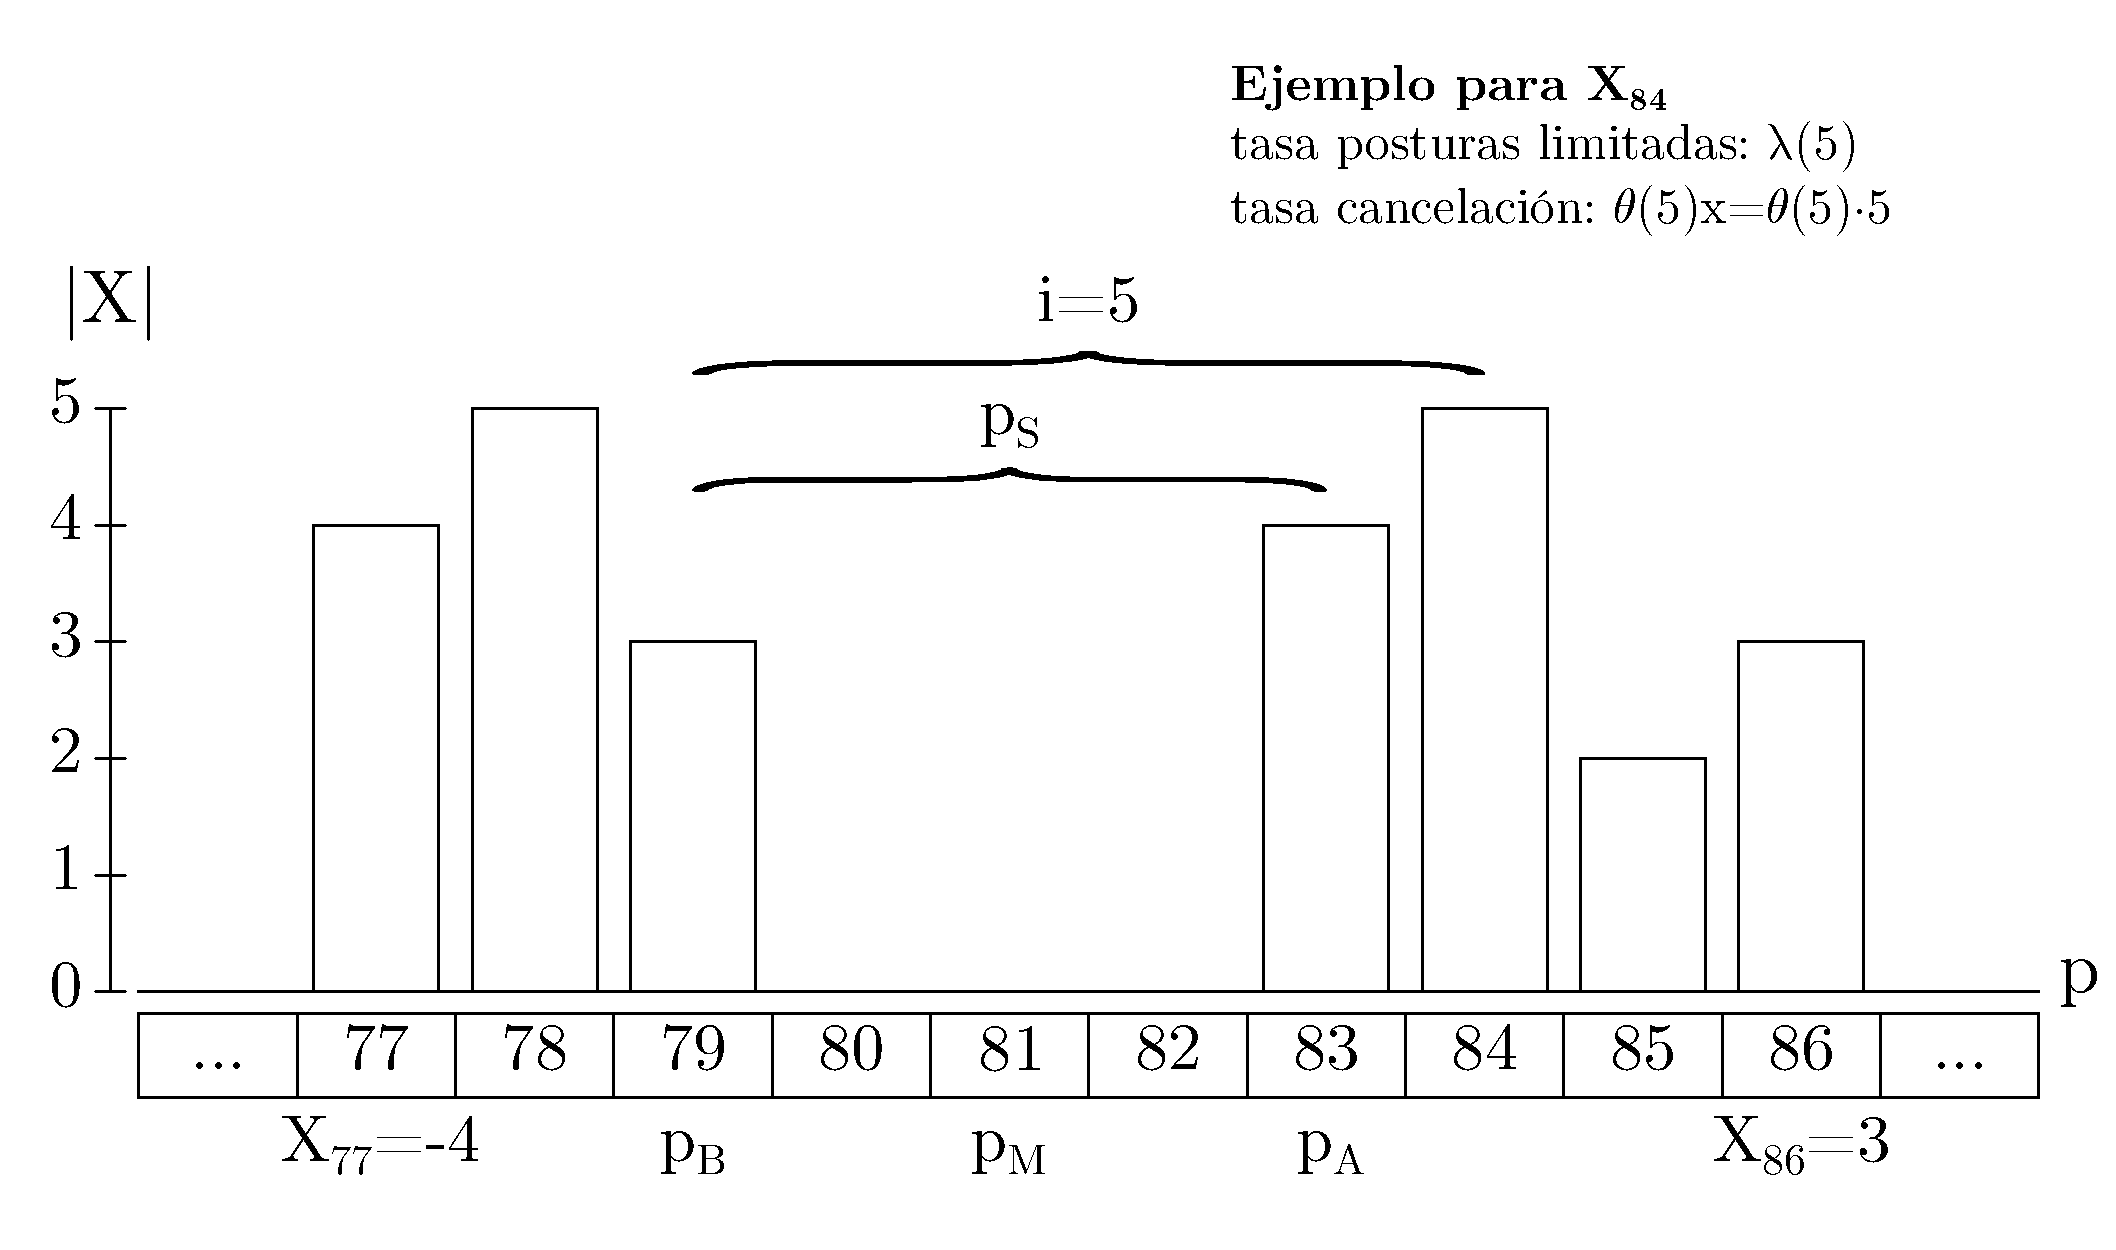
\includegraphics[scale=0.38,trim=0 1cm 0 1cm]{model.pdf}
\caption{Diagrama del modelo}
\label{model}
\end{figure}

\subsection{Dirección de los Movimientos en el Precio}

Se desea calcular la probabilidad de que en el siguiente movimiento el precio medio $p_M(t)$ aumente. El precio medio se altera en el tiempo del primer paso de las colas al mejor precio de compra o venta a cero. También este precio se puede alterar si el ``spread'' $p_S(t)>1$ y llega una postura dentro de este ``spread''. Se define a $X_A=X_{p_A(\cdot)}(\cdot)$ y $X_B=X_{p_B(\cdot)}(\cdot)$ y $\tau=\inf\{t\geq 0, p_M(t) \neq p_M(0)\}$.\\

Dada una configuración inicial del libro de posturas y un ``spread'' inicial $S$, la probabilidad de que en el siguiente movimiento el precio medio aumente se puede expresar de la siguiente forma:
\[
P\{p_M(\tau)>p_M(0)|X_A(0)=a,X_B(0)=b,p_S(0)=S\}
\]

Los procesos $X_A$ y $X_B$ son procesos de nacimiento y muerte con las siguientes tasas de transición:
\[
n\rightarrow n+1 \text{ con una tasa }\lambda(S)
\]
\[
n\rightarrow n-1 \text{ con una tasa }\mu+n\theta(S)
\]\\

En particular cuando $S=1$ el precio medio $p_M(t)$ se altera cuando $X_A$ ó $X_B$ alcanzan el estado 0. Ahora, si se denota $\sigma_A$ y $\sigma_B$ como el tiempo del primer paso de los procesos $X_A$ y $X_B$ a cero, la distribución de $\tau$ está dada por el mínimo de los tiempos del primer paso a cero de los procesos $X_A$ y $X_B$. La probabilidad de interés se puede expresar como $P\{\sigma_A<\sigma_B|X_A(0)=a,X_B(0)=b,p_S(0)=S\}$. La transformación de Laplace de la distribución condicional de $\sigma_A-\sigma_B$ está dada por:
\[
\hat{f}_a^1(s)\hat{f}_b^1(-s)
\]
donde como se puede ver en el Apéndice \ref{eq:fidist}:
\[
\hat{f}_{j}^S(s)=\left(-\frac{1}{\lambda(S)}\right)^j\left( \prod_{i=1}^j \Phi_{k=i}^\infty \frac{-\lambda(S)(\mu+k\theta(S))}{\lambda(S)+\mu+k\theta(S)+s} \right)
\]\\

Por lo que la probabilidad buscada se obtiene al evaluar la función de distribución acumulada en 0. Para hacer esto es necesario encontrar la transformación inversa de $\hat{f}_a^1(s)\hat{f}_b^1(-s)$ e integrar esta función.\\

En el caso de que $S>1$, es necesario considerar que si se recibe una postura dentro del spread el precio medio $p_M(t)$ también se alterará. Por lo que si se denota $\sigma_A^i$ y $\sigma_B^i$ como el tiempo en el que llega la primera orden a $i$ pujas del mejor precio de venta o compra respectivamente; el tiempo en el que cambia por primera vez $p_M(t)$ está dado por el mínimo de los tiempos $\sigma_A,\sigma_B,\sigma_A^i$ y $\sigma_B^i$ con $i=1,\ldots,S-1$. Es importante mencionar que $\sigma_A^i$ y $\sigma_B^i$ se distribuyen de manera exponencial con tasa $\lambda(i)$. Para que $p_M(t)$ aumente es necesario que arribe una orden de compra a $S-1$ pujas del mejor precio de venta o se agoten las posturas al mejor precio de venta antes de que llegue una postura de venta a $S-1$ pujas de la mejor postura de compra o se agoten las posturas al mejor precio de compra.\\

En este caso la probabilidad buscada está dada por $P\{\sigma_A \land \sigma_B^1 \land \cdots \land \sigma_B^{S-1} < \sigma_B \land \sigma_A^1 \land \cdots \land \sigma_A^{S-1}|X_A(0)=a,X_B(0)=b,p_S(0)=S\}$. El mínimo de un conjunto de variables aleatorias que se distribuyen de forma exponencial con parámetros $\lambda_1,\ldots,\lambda_n$ tiene una distribución exponencial con parámetro $\lambda_1+\ldots+\lambda_n$. Por lo que se puede expresar la probabilidad de interés de la siguiente forma $P\{\sigma_A \land \sigma_B^\Sigma < \sigma_B \land \sigma_A^\Sigma|X_A(0)=a,X_B(0)=b,p_S(0)=S\}$ donde $\sigma_A^\Sigma$ y $\sigma_B^\Sigma$ son
variables aleatorias exponenciales independientes con tasa $\Lambda_S$. Por lo que se puede probar, que la transformación de Laplace de la función de densidad de $\sigma_A \land \sigma_B^\Sigma - \sigma_B \land \sigma_A^\Sigma$ está dada por \cite{Cont2010}:
\[
\resizebox{\hsize}{!}{$
\left(\hat{f}_a^S(\Lambda_S+s)+\frac{\Lambda_S}{\Lambda_S+s}(1-\hat{f}_a^S(\Lambda_S+s))\right)
\left(\hat{f}_b^S(\Lambda_S+s)+\frac{\Lambda_S}{\Lambda_S+s}(1-\hat{f}_b^S(\Lambda_S+s))\right)
$}
\]
donde $\Lambda_S=\sum_{i=1}^{S-1}\lambda(i)$. De igual forma es necesario encontrar la transformación, integrar la función y evaluar en 0.\\

\subsection{Retos de la Transformación Inversa de Laplace}
\label{sec:retos}

Los métodos para invertir la transformación de Laplace discutidos en la sección anterior están diseñados para la transformación unilateral de Laplace, es decir definida en los reales positivos. La distribución de  $\sigma_A \land \sigma_B^\Sigma - \sigma_B \land \sigma_A^\Sigma$ están definidas en todos los reales, por lo que es necesario utilizar algunas herramientas para poder encontrar la transformación inversa.\\

Es importante tener presente que el método utilizado para encontrar la transformación inversa presentado en este trabajo está basado en la expansión en series de Fourier, el cual utiliza funciones pares. Además es importante notar que el método permite encontrar la transformación inversa para $t \in (0,T)$. Las funciones de densidad estudiadas no son pares y están definidas para $t<0$ por lo que para resolver este problema se define la función $g(t)=
f(t-a)$, donde $a$ es tal que:
\[
\lim_{t\to 0^-} g(t)=0
\]

El objetivo de la función $g$ es truncar la distribución $f$ y desplazarla de tal forma que los datos que se omiten no sean representativos. Es importante recordar que como $f$ es una función de distribución $f(t)\geq 0$ para toda $t$ en el dominio de la función.\\

En este caso se realizaron diversas simulaciones de los procesos $X_A$ y $X_B$ para evaluar la distribución de $\tau$, la cual disminuye exponencialmente de ambos lados a partir de un cierto máximo. En la Figura \ref{probmt} se muestra el resultado que se obtiene de las simulaciones y el que se obtiene al utilizar el método de la transformación inversa de Laplace.\\

\begin{figure}[htbp] \centering
\includegraphics[scale=0.75,trim=0 1cm 0 1cm]{probpm.eps}
\caption{Comparación de la función de densidad de $\tau$ obtenida por simulación y por la transformación inversa de Laplace}
\label{probmt}
\end{figure}

Si se define a $u(t)$ como la función de escalón unitario, es decir:
\[
u(t) =
\begin{cases}
0, & \mbox{si } x<0 \\
1, & \mbox{si } x\geq0
\end{cases}
\]
debido a las propiedades de la transformación de Laplace:
\[
\mathcal{L} \left\{g(t)u(t-a)\right\}=\mathcal{L} \left\{f(t-a)u(t-a)\right\}=e^{-as}\hat{f}(s)
\]
por lo que de esta forma se puede desplazar la función de densidad de forma que $\lim_{t\to 0^-} g(t)=0$, como se puede apreciar en la Figura \ref{probmtshift}.\\

\begin{figure}[htbp] \centering
\includegraphics[scale=0.75,trim=0 1cm 0 1cm]{probpmshift.eps}
\caption{Desplazamiento de la función de densidad de $\tau$}
\label{probmtshift}
\end{figure}

También es importante utilizar el parámetro apropiado $T$ para encontrar la distribución de la mejor manera posible. Como se puede ver en la Figura \ref{probmtpar}, la función de densidad es radicalmente distinta cuando $T$ no es lo suficientemente grande.

\begin{figure}[htbp] \centering
\includegraphics[scale=0.75,trim=0 1cm 0 1cm]{probpmpar.eps}
\caption{Función de densidad de $\tau$ para distintos parámetros $T$}
\label{probmtpar}
\end{figure}

\clearpage

\subsection{Estimación de los Parámetros}

En este trabajo se utilizan los parámetros propuestos en \cite{Cont2010}; debido a que el modelo considera posturas con un volumen estandarizado o único, es necesario encontrar el promedio de las posturas limitadas $S_l$, posturas a mercado $S_m$ y de las cancelaciones $S_c$. Con esto se estima la tasa de llegada de las ordenes limitadas $\lambda$ a una distancia de $i$ pujas, $1\leq i \leq 5$:

\[
\hat{\lambda}(i)=\frac{N_l(i)}{T_*}
\]
donde $N_l(i)$ es el número de posturas que llegaron a una distancia $i$ de la mejor postura contraria y $T_*$ es el tiempo total en el que el mercado estuvo abierto expresado en minutos. Este es el estimador de máxima verosimilitud de una distribución Poisson el cual es insesgado. Para $i>5$ esto se extrapola siguiendo la siguiente ley de potencias:
\[
\hat{\lambda}(i)=\frac{k}{i^\alpha}
\]\\
donde $k$ y $\alpha$ son los parámetros que minimizan el error cuadrático medio para $1\leq i \leq 5$.\\

La tasa de llegada de las posturas a mercado $\mu$ se estima de la siguiente forma:
\[
\hat{\mu}=\frac{N_m}{T_*}\frac{S_m}{S_l}
\]
$N_m$ es el número de posturas de mercado; en este caso se consideran como posturas de mercado todas aquellas que superan la mejor postura contraria. Este estimador es similar a el de $\lambda$, sólo que se ajusta por las diferencias entre los volúmenes estandarizados de las órdenes limitadas y las de mercado.\\

En trabajos anteriores no se cuenta con información tan detallada del libro de posturas, por lo que no se han considerado las modificaciones que en este caso forman una parte muy importante de la muestra. El promedio del volumen de las modificaciones para BIMBO es casi 10 veces mayor al de las nuevas posturas. Esto se puede deber a que los participantes del mercado que están interesados en comprar o vender un volumen mayor seguramente lo harán a través de posturas limitadas, ya que son más sensibles al precio. Las posturas limitadas garantizan un precio, mientras que a través de una postura a mercado se garantiza la ejecución pero no el precio. Los participantes con posturas de gran volumen se verán obligados a adaptar el precio de sus posturas a través de modificaciones para lograr la ejecución de las mismas. Existen tres alternativas:
\begin{itemize}
  \item Considerar las modificaciones como una cancelación y una nueva postura
  \item Ignorar las modificaciones
  \item Modelar las modificaciones como otro proceso\\
\end{itemize}

La primera alternativa es la que más se acerca a estudios anteriores ya que estos no cuentan con la noción de las modificaciones, al tener la información de las puntas del libro de posturas sólo notan la cancelación de una postura y la aparición de una nueva a otro nivel. No se considera la diferencia en el volumen de las nuevas posturas y de las modificaciones. Por ejemplo, en la acción de BIMBO el volumen de las nuevas posturas limitadas de compra es de 2,005.23. Mientras que si se toman en conjunto las nuevas posturas y las modificaciones el promedio del volumen es de 10,518.09. Esto se debe a que el promedio del volumen de las modificaciones de compra es de 27,237.23. La segunda alternativa no es viable ya que hay un gran número de modificaciones, al ignorarlas se descartaría información importante en el modelo. La tercera alternativa le agrega un poco de complejidad al modelo, ya que es necesario modelar de alguna forma la llegada de las modificaciones y el comportamiento de ellas. En este caso se optará por la primera alternativa.\\

Finalmente para calcular los parámetros de cancelación $\theta(i)$, es necesario calcular el libro promedio debido a que bajo los supuestos del modelo, el número de cancelaciones depende del número de órdenes activas. El libro promedio es el promedio del volumen de compra (venta) a una distancia de $i$ pujas de la mejor postura contraria. En la Figura \ref{fig:bookavg} se encuentra el libro promedio para BIMBO. Si se define $Q_i^A$ y $Q_i^B$ como el número promedio de órdenes activas a $i$ pujas de la mejor postura de venta y compra respectivamente,  $\theta(i)$ para $1\leq i \leq 5$ se pueden calcular de la siguiente forma, donde $Q_i$ es el promedio de $Q_i^A$ y $Q_i^B$:
\[
\hat{\theta}(i)=\frac{N_c(i) S_c}{Q_i T_*}
\]
$N_c(i)$ es el número de posturas de cancelación a una distancia $i$ de la mejor postura contraria. Para $i>5$, $\hat{\theta}(i)=\hat{\theta}(5)$.\\

\begin{figure}[htbp]
\centering
\begin{subfigure}[b]{0.5\textwidth}
\centering
\includegraphics[width=\textwidth, trim=0 0.5cm 0 1cm]{compraavg.eps}
\caption{BIMBO compra promedio}
\label{fig:compraavg}
\end{subfigure}%
~ %add desired spacing between images, e. g. ~, \quad, \qquad etc.
%(or a blank line to force the subfigure onto a new line)
\begin{subfigure}[b]{0.5\textwidth}
\centering
\includegraphics[width=\textwidth, trim=0 0.5cm 0 1cm]{ventaavg.eps}
\caption{BIMBO venta promedio}
\label{fig:ventavg}
\end{subfigure}
%add desired spacing between images, e. g. ~, \quad, \qquad etc.
%(or a blank line to force the subfigure onto a new line)

\caption{Libro Promedio}
\label{fig:bookavg}
\end{figure}

Al realizar los cálculos antes descritos para la emisora BIMBO se obtienen los parámetros que se encuentran en la Tabla \ref{tab:paremeters}.

\begin{table}[htbp]
\centering
\caption{Parámetros del Modelo}
\begin{tabular}{r|r|r|r|r|r|}
\cline{2-6}
& 1& 2 & 3 & 4 & 5 \\
\cline{2-6}
$\lambda(i)$ & 0.1669 & 0.0732 & 0.0655 & 0.0601 & 0.0731 \\
$\theta(i)$ & 0.6480 & 0.9954 & 1.3240 & 1.5714 & 0.7582 \\
\cline{2-6}
$\mu$ & 0.1438 & & & & \\
\cline{2-6}
\end{tabular}%
\label{tab:paremeters}%
\end{table}%

\clearpage

\subsection{Resultados}

Para entender los resultados, en primer lugar, es necesario obtener las probabilidades empíricas para compararlas con las obtenidas por el modelo. En este caso, se eligió la acción de BIMBO, en particular los casos donde $S=1$, es decir, la distancia de la mejor postura de compra a la mejor postura de venta es de 1 puja. Para el caso de BIMBO, existen 21,256 eventos donde $S=1$ de los 173,616 eventos que sucedieron en los 68 días de estudio.

\begin{table}[htbp]
  \centering
  \caption{Ejemplo: Posturas BIMBO}
    \begin{tabular}{rrrrrrrrrrr}
    id    & timestamp &       & $p_B(t)$    & $X_{p_B}(t)$ &       & $p_A(t)$    & $X_{p_A}(t)$   &       & $S$     & $p_M(t)$ \\
    151   & 1289919878430 &       & 97.79 & 600   &       & 97.8  & 2100  &       & 1  & 97.7950 \\
    152   & 1289919878450 &       & 97.79 & 600   &       & 97.8  & 2100  &       & 1  & 97.7950 \\
    153   & 1289919882930 &       & 97.79 & 600   &       & 97.8  & 1500  &       & 1  & 97.7950 \\
    154   & 1289919882940 &       & 97.79 & 600   &       & 97.8  & 1500  &       & 1  & 97.7950 \\
    155   & 1289919883070 &       & 97.75 & 39000 &       & 97.79 & 900   &       & 4  & 97.7700 \\
    \end{tabular}%
  \label{tab:bimbotab}%
\end{table}%

Para analizar los resultados, se considerará la primera postura donde $S=1$, en el ejemplo de la Tabla \ref{tab:bimbotab} esto sucede en el renglón 151, donde $p_M(t)$ es 97.7950 y el volumen de la mejor postura de venta excede el de la mejor postura de compra. Los siguientes eventos modifican posturas distintas a las puntas o el volumen en las puntas, hasta el evento 155 donde se modifica $p_M(t)$.\\

Para la acción de BIMBO existen 2,196 instancias como esta; para poder realizar el análisis se encontró la media del volumen del primer evento de cada instancia donde $S=1$, la cual es de 2,707.45. El volumen de todos los eventos se dividió entre la media y se tomó el número entero más cercano mayor a este cociente para realizar los cálculos. Para el análisis se consideran las posturas donde el volumen normalizado es menor o igual que 5. De las 2,196 instancias mencionadas antes 2,043 cumplen esto; éstas se muestran en la Tabla \ref{tab:numempirca}. En la Tabla \ref{tab:numempirca} las columnas muestran posturas de venta con volúmenes normalizados de 1 a 5 y los renglones posturas de compra con volúmenes normalizados de 1 a 5.\\

\begin{table}[htbp]
\centering
\caption{Número de Posturas}
\begin{tabular}{r|p{1.5cm}|p{1.5cm}|p{1.5cm}|p{1.5cm}|p{1.5cm}|}
\multicolumn{6}{c}{venta}\\
\cline{2-6}
compra & 1& 2 & 3 & 4 & 5 \\
\cline{2-6}
1 & 1,217 & 253 & 116 & 59 & 5 \\
2 & 193 & 23 & 9 & 4 & 1 \\
3 & 62 & 3 & 4 & 1 & 1 \\
4 & 39 & 4 & 0 & 0 & 0 \\
5 & 15 & 1 & 0 & 0 & 0 \\
\cline{2-6}
\end{tabular}%
\label{tab:numempirca}%
\end{table}%

En la Tabla \ref{tab:resempirca} se encuentran los resultados que se obtuvieron. Esta tabla es similar a la Tabla  \ref{tab:numempirca}. Por lo que, por ejemplo, en el renglón 3 con la columna número 1 se dice que cuando existen 3 posturas estandarizadas de compra y una postura estandarizada de venta, la probabilidad de que el precio aumente es del 67.74\%. En los casos donde existen el mismo número de posturas de compra que de venta los resultados no son muy claros, ya que sólo en el 39.93\% y 34.78\% para 1 y 2 posturas respectivamente aumenta el precio; se esperaría un número cercano al 50\%. Sin embargo, los resultados sí reflejan algo que se esperaría, en los casos donde el número de posturas de compra es mayor que el número de posturas de venta la probabilidad de un aumento de precio es mayor; al aumentar esta diferencia aumenta también la probabilidad de que el precio suba. Muchas de las combinaciones son poco concluyentes, ya que la muestra es muy pequeña.

\begin{table}[htbp]
\centering
\caption{Resultados Empíricos}
\begin{tabular}{r|p{1.5cm}|p{1.5cm}|p{1.5cm}|p{1.5cm}|p{1.5cm}|}
\multicolumn{6}{c}{venta}\\
\cline{2-6}
compra & 1& 2 & 3 & 4 & 5 \\
\cline{2-6}
1 & 39.93\% & 11.86\% & 9.48\% & 11.86\% & 2.63\% \\
2 & 60.62\% & 34.78\% & 11.11\% & 50.00\% & 0.00\% \\
3 & 67.74\% & 33.33\% & 75.00\% & 0.00\% & 100.00\% \\
4 & 76.92\% & 25.00\% & - & - & - \\
5 & 93.33\% & 0.00\% & - & - & - \\
\cline{2-6}
\end{tabular}%
\label{tab:resempirca}%
\end{table}%

Los resultados obtenidos al aplicar el método de la transformación de Laplace siguen una tendencia similar como se puede ver en la Tabla \ref{tab:reslaplace}, la cual se interpreta de manera similar a la Tabla \ref{tab:resempirca}. En este caso cuando el número de órdenes de compra es el mismo al de las de venta, la probabilidad de un aumento en $p_M(t)$ es cercana al 50\%. Cuando el número de posturas de compra excede al de venta existe una mayor probabilidad de que el precio suba para todos los casos; también al aumentar la diferencia entre las posturas de compra y venta aumenta la probabilidad de un aumento en el precio. Un resultado interesante es que se esperaría que $P\{p_M(T)>p_M(0)|X_A(0)=a,X_B(0)=b,p_S(0)=1\}=1-P\{p_M(T)>p_M(0)|X_A(0)=b,X_B(0)=a,p_S(0)=1\}$; sin embargo, en este caso $P\{p_M(T)>p_M(0)|X_A(0)=1,X_B(0)=2,p_S(0)=1\}=69.31\%$ mientras que $P\{p_M(T)>p_M(0)|X_A(0)=2,X_B(0)=1,p_S(0)=1\}=35.32\%$. Esto se puede deber a la precisión de algunos de los cálculos que se realizaron, en particular las integraciones numéricas; esto se podría mejorar al alterar los parámetros.\\

\begin{table}[htbp]
\centering
\caption{Resultados de la Transformación de Laplace}
\begin{tabular}{r|p{1.5cm}|p{1.5cm}|p{1.5cm}|p{1.5cm}|p{1.5cm}|}
\multicolumn{6}{c}{venta}\\
\cline{2-6}
compra & 1& 2 & 3 & 4 & 5 \\
\cline{2-6}
1 & 53.49\% & 35.32\% & 26.21\% & 20.82\% & 17.27\% \\
2 & 69.31\% & 52.28\% & 41.79\% & 34.75\% & 29.73\% \\
3 & 77.16\% & 62.26\% & 52.02\% & 44.60\% & 39.01\% \\
4 & 81.81\% & 68.80\% & 59.22\% & 51.91\% & 46.17\% \\
5 & 84.89\% & 73.42\% & 64.55\% & 57.52\% & 51.85\% \\
\cline{2-6}
\end{tabular}%
\label{tab:reslaplace}%
\end{table}%

Con los mismos parámetros que se utilizaron para el método de Laplace se realizaron simulaciones. Para cada una de las combinaciones se realizaron 10,000 simulaciones en el paquete estadístico R; los resultados se \DIFdelbegin \DIFdel{muestra }\DIFdelend \DIFaddbegin \DIFadd{muestran }\DIFaddend en la Tabla \ref{tab:ressim}. Para las simulaciones en los casos donde el número de posturas de compra y venta son iguales, el porcentaje de las ocasiones donde el precio sube es el más cercano al 50\%. También en este método se cumplen las premisas que se establecieron en los otros dos métodos en cuanto al aumento de la probabilidad de que el precio suba dada la diferencia entre el número de posturas de compra y venta. En este caso se podría decir que $P\{p_M(T)>p_M(0)|X_A(0)=a,X_B(0)=b,p_S(0)=1\}=1-P\{p_M(T)>p_M(0)|X_A(0)=b,X_B(0)=a,p_S(0)=1\}$ sí se cumple. Este método resultó ser bastante más rápido que el método de la transformación inversa de Laplace, sin embargo, probablemente el método de Laplace se podría mejorar considerablemente si se optimizaran algunos de los algoritmos utilizados. Por ejemplo, el algoritmo utiliza los mismos resultados en varias ocasiones, por lo que estos se podrían almacenar para evitar calcularlos en cada ocasión.

\begin{table}[htbp]
\centering
\caption{Resultados Simulación}
\begin{tabular}{r|p{1.5cm}|p{1.5cm}|p{1.5cm}|p{1.5cm}|p{1.5cm}|}
\multicolumn{6}{c}{venta}\\
\cline{2-6}
compra & 1& 2 & 3 & 4 & 5 \\
\cline{2-6}
1 & 49.85\% & 33.23\% & 25.10\% & 19.71\% & 16.29\% \\
2 & 66.78\% & 50.26\% & 40.35\% & 33.20\% & 28.28\% \\
3 & 75.55\% & 60.08\% & 50.41\% & 42.41\% & 36.89\% \\
4 & 79.55\% & 66.27\% & 57.13\% & 49.40\% & 43.76\% \\
5 & 83.90\% & 71.98\% & 63.65\% & 55.75\% & 50.59\% \\
\cline{2-6}
\end{tabular}%
\label{tab:ressim}%
\end{table}%

\clearpage

\section{Conclusiones}

En el trabajo se reconstruyó el libro de posturas de la Bolsa Mexicana de Valores, el algoritmo logró reproducir con gran eficacia los hechos reportados por la BMV, medidos desde el punto de vista del volumen y del VWAP.\\

Se compararon los resultados obtenidos con los análisis que se han realizado para otros mercados. Para algunas de las variables los resultados fueron similares a los encontrados en otros mercados; por ejemplo los precios siguen una ley de potencias. También se puede decir que el volumen de las órdenes sigue la ley de potencias, sin embargo, las cancelaciones no tienen un comportamiento similar. La mayoría de las cancelaciones suceden cerca de las puntas.\\

En el trabajo se describió un modelo del libro de posturas simplificado, el cual clasifica las órdenes en: órdenes limitadas, de mercado y cancelaciones, a las cuales les asigna una distinta tasa de llegada. El modelo tiene la bondad de permitir el cálculo de algunos resultados a través de la transformación inversa de Laplace, la cual facilita los mismos debido a sus propiedades.\\

El trabajo se concentró en describir el comportamiento de los movimientos del precio. Para realizar los cálculos necesarios se utilizó el método de Laplace y una expresión de la probabilidad buscada en términos de fracciones continuas. Para realizar los cálculos fue necesario estimar los parámetros. Para poder comparar los resultados obtenidos a través del método de Laplace, se realizaron los cálculos de las frecuencias empíricas y a través de simulación.\\

En particular se calculó la probabilidad de un aumento en el precio cuando el ``spread'' es de una puja; las frecuencias empíricas muestran algunas diferencias con los resultados obtenidos a través de la transformación de Laplace y simulación, sin embargo los resultados eran consistentes con los que se esperaban; al aumentar la diferencia entre las posturas de compra y venta, aumenta la probabilidad de que aumente el precio. El método de la transformación de Laplace resultó ser significativamente más lento que las simulaciones.\\

En trabajos futuros se podría probar el método de la transformación inversa en casos donde el ``spread'' es mayor que 1, para estos casos podría ser que este método fuera más veloz que la simulación. También se deja para un trabajo posterior la implementación de estrategias para explotar los resultados encontrados en el trabajo. Para implementar estas estrategias es necesario optimizar los algoritmos utilizados en este trabajo.\\

El modelo utilizado también puede ser perfeccionado; en particular se podría eliminar el supuesto de órdenes de un tamaño unitario o estándar. También se podrían utilizar distintos parámetros para las órdenes de compra y venta.


\clearpage

\appendix
\section{Apéndice} \label{App:AppendixA}
% the \\ insures the section title is centered below the phrase: AppendixA

Se considera que la base matemática necesaria para el modelo que se desarrolló anteriormente puede ser valiosa para el lector, por lo que a continuación se presenta en forma exhaustiva. Primero, se describen los procesos estocásticos de nacimiento y muerte; luego, se encuentra la distribución de los tiempos de transición mediante la transformación de Laplace y fracciones continuas.\\

\subsection{Procesos Estocásticos y Tiempos de Transición}

En esta sección se define formalmente el concepto de cadena de Markov homogénea y un caso particular de éstos; los procesos de nacimiento y muerte. Un proceso estocástico $\{X(t);t\geq 0\}$ con un conjunto de estados \DIFdelbegin \DIFdel{$\mathcal{S} \subset I$ }\DIFdelend \DIFaddbegin \DIFadd{$\mathcal{S} \subset \mathbb{N}$ }\DIFaddend se dice que es una cadena de Markov de tiempo continuo si para toda $n \in \mathbb{N}$, estados $i_{1},i_{2},\ldots,i_{n},j$; tiempos $0\leq\tau_0<\tau_1<\cdots<\tau_n<\tau$:

\[
P\{X(\tau)=j|X(\tau_1)=i_1\ldots X(\tau_n)=i_n\}
\]
\begin{equation}
= P\{X(\tau)=j|X(\tau_n)=i_n\}
\end{equation}

Una cadena de Markov de tiempo continuo es homogénea, si para toda $0\leq s <\tau$:
\begin{equation}
P\{X(\tau)=j|X(s)=i\}=P\{X(\tau-s)=j|X(0)=i\}
\end{equation}

Un proceso estocástico se conoce como proceso de nacimiento y muerte con un espacio de estados $\mathcal{S}$, si cumple con los siguientes axiomas:

\begin{enumerate}
  \item \DIFdelbegin \DIFdel{$\mathcal{S} \subset I = \{ 0,1,2,\ldots\}$
  }\DIFdelend \DIFaddbegin \DIFadd{$\mathcal{S} \subset \mathbb{N}$
  }\DIFaddend \item Es una cadena de Markov homogénea
  \item Existen las constantes no negativas $\lambda_j$ y $\mu_j$, con $j=0,1,\ldots$ con $\mu_0=0$, tal que para $s>0$ y $t\geq 0$, se cumple:
\begin{subequations}
\begin{eqnarray}
P\{X(t+s)-X(t)=1|X(t)=j\} = \lambda_j s + o(s)\quad j \in I \\
P\{X(t+s)-X(t)=-1|X(t)=j\} = \mu_js + o(s)\quad j \in I \\
P\{\left|X(t+s)-X(t)\right|>1|X(t)=j\} = o(s)\quad j \in I \\
P\{X(t+s)=j|X(t)=j\} = 1-(\lambda_j+\mu_j)s + o(s)\quad j \in I 
\end{eqnarray}
\end{subequations}
\end{enumerate}


$X(t)$ se conoce como el tamaño de la población al tiempo $t$. A $\lambda_j$ se le conoce como la tasa de nacimiento y $\mu_j$ como la tasa de muerte. Una medida interesante de los procesos de nacimiento y muerte es el tiempo del primer paso del estado $i$ al estado $j$, que se denota como $\sigma_{i,j}$. Para calcular la distribución de esta variable aleatoria es conveniente utilizar la transformación de Laplace bilateral, la cual se define de la siguiente forma:

\begin{equation}
\hat{f}(s) = \mathcal{L} \left\{f(t)\right\}=\int_{-\infty}^{\infty} e^{-st} f(t) \,dt
\end{equation}\\

De aquí en adelante se referirá a la transformación bilateral de Laplace simplemente como la transformación de Laplace.\\

El tiempo $\sigma_{i,j}$ se puede expresar de la siguiente forma:
\begin{equation}
\sigma_{i,j}=\sigma_{i,i+1}+\sigma_{i+1,i+2}+\ldots+\sigma_{j-1,j}
\end{equation}
donde $\sigma_{k,k+1}$ con $k=1,2,\ldots,j-1$ son independientes, lo cual permite utilizar la siguiente propiedad de la transformación de Laplace:
\begin{equation}
\mathcal{L} \left\{f_{X+Y}(t)\right\}=\hat{f}_{X+Y}(s)=\operatorname{E}[e^{-s(X+Y)}]
\end{equation}

\begin{equation}
\operatorname{E}[e^{-s(X+Y)}]=\operatorname{E}[e^{-sX}]\operatorname{E}[e^{-sY}]=\hat{f}_{X}(s)\hat{f}_{Y}(s)
\end{equation}

La transformación de la función de densidad de $\sigma_{i,j}$ se puede expresar como:
\begin{equation} \label{eq:laplacesum}
\mathcal{L} \left\{\sigma_{i,j}(t)\right\}=\hat{f}_{i,j}(s)=\prod_{k=i}^{j-1}\hat{f}_{k,k+1}(s)
\end{equation}
haciendo deseable encontrar una transformación $\mathcal{L}^{-1}$ tal que:
\begin{equation}
\mathcal{L}^{-1}\{\hat{f}(s)\}=f(t)
\end{equation}

Primero es necesario encontrar una expresión para $\hat{f}_{i,i-1}$. Ahora, si se condiciona $\sigma_{i,i-1}$ a la primera transición, donde $S_1$ es el tiempo para el primer evento, se puede expresar como:

\begin{equation}
\sigma_{i,i-1} =
\begin{cases}
S_{1}, & \mbox{si } X(S_{1})=i-1 \\
S_{1}+\sigma_{i+1,i-1}, & \mbox{si } X(S_{1})=i+1
\end{cases}
\end{equation}
\begin{equation}
\sigma_{i+1,i-1}=\sigma_{i+1,i}+\sigma_{i,i-1}
\end{equation}

\[
\begin{array}{rcrcl}
F_{i,i-1}(t) & = & P\{ \sigma_{i+1,i-1}\leq t \} & = & P\{ \sigma_{i,i-1}\leq t | X(S_{1})=i-1 \}P\{ X(S_{1})=i-1 \} +\\
 & & & & P\{ \sigma_{i,i-1}\leq t | X(S_{1})=i+1 \}P\{ X(S_{1})=i+1 \} \\
 & & & = & P\{ S_{1}\leq t\}P\{ X(S_{1})=i-1 \} +\\
 & & & & P\{ S_{1} + \sigma_{i+1,i-1}\leq t\}P\{ X(S_{1})=i+1 \} \\
 & & & = & \frac{\mu_{i}}{\lambda_{i}+\mu_{i}} P\{ S_{1}\leq t\} + \frac{\lambda_{i}}{\lambda_{i}+\mu_{i}} P\{ S_{1} + \sigma_{i+1,i-1}\leq t\}\\
 & & & = & \frac{\mu_{i}}{\lambda_{i}+\mu_{i}} F_{S_{1}}(t) + \frac{\lambda_{i}}{\lambda_{i}+\mu_{i}} F_{ S_{1} + \sigma_{i+1,i-1}}(t)\\
\end{array}
\]

\[
\begin{array}{rcrcl}
\frac{d}{dt} F_{i,i-1}(t) & = & f_{i,i-1}(t) & = & \frac{\mu_{i}}{\lambda_{i}+\mu_{i}} \frac{d}{dt} F_{S_{1}}(t) + \frac{\lambda_{i}}{\lambda_{i}+\mu_{i}} \frac{d}{dt} F_{ S_{1} + \sigma_{i+1,i-1}}(t)\\
 & & & = & \frac{\mu_{i}}{\lambda_{i}+\mu_{i}} f_{S_{1}}(t) + \frac{\lambda_{i}}{\lambda_{i}+\mu_{i}} f_{ S_{1} + \sigma_{i+1,i-1}}(t)\\
\end{array}
\]

Ahora $S_1$ tiene una distribución exponencial con media $\frac{1}{\lambda_i+\mu_i}$ por lo que:
\[
\mathcal{L}\{f_{S_1}(t)\}=\int_{0}^{\infty} e^{-st} f_{S_1}(t)\,dt=(\lambda_i+\mu_i)\int_{0}^{\infty} e^{-(\lambda_i+\mu_i+s)t}\,dt=\frac{\lambda_i+\mu_i}{\lambda_i+\mu_i+s}
\]

\[
\begin{array}{rcrcl}
\mathcal{L} \{ f_{i,i-1}(t) \} & = & \hat{f}_{i,i-1}(s) & = & \mathcal{L} \{ \frac{\mu_{i}}{\lambda_{i}+\mu_{i}} f_{S_{1}}(t) + \frac{\lambda_{i}}{\lambda_{i}+\mu_{i}} f_{ S_{1} + \sigma_{i+1,i-1}}(t) \}\\
 & & & = & \frac{\mu_{i}}{\lambda_{i}+\mu_{i}} \hat{f}_{S_{1}}(s) + \frac{\lambda_{i}}{\lambda_{i}+\mu_{i}} f_{ S_{1} + \sigma_{i+1,i-1}}(s) \\
 & & & = & \frac{\mu_{i}}{\lambda_{i}+\mu_{i}} \frac{\lambda_{i}+\mu_{i}}{\lambda_{i}+\mu_{i}+s} + \frac{\lambda_{i}}{\lambda_{i}+\mu_{i}} \hat{f}_{S_{1}}(s) \hat{f}_{\sigma_{i+1,i}}(s) \hat{f}_{\sigma_{i,i-1}}(s) \\
 & & & = & \frac{\mu_{i}}{\lambda_{i}+\mu_{i}} \frac{\lambda_{i}+\mu_{i}}{\lambda_{i}+\mu_{i}+s} + \frac{\lambda_{i}}{\lambda_{i}+\mu_{i}} \frac{\lambda_{i}+\mu_{i}}{\lambda_{i}+\mu_{i}+s} \hat{f}_{i+1,i}(s) \hat{f}_{i,i-1}(s) \\
\end{array}
\]

\begin{equation} \label{eq:distgen}
\hat{f}_{i,i-1}(s) = \frac{\mu_{i}}{\lambda_{i}+\mu_{i}+s-\lambda_{i}\hat{f}_{i+1,i}(s)}
\end{equation}\\

Otro concepto que es necesario introducir es lo que se conoce como fracciones continuas. Las cuales son expresiones de la forma:
\[
\cfrac{a_1}{b_1 + 
\cfrac{a_2}{b_2 + 
\cfrac{a_3}{b_3+ \ddots}}}
\]

Una fracción continua infinita se define con las sucesiones $\left[\{a_n\}_1^{\infty},\{b_n\}_1^{\infty}\right]$ donde $t_k$ se define como:
\[
t_k:\rightarrow \frac{a_k}{b_k+u}
\]
donde:
\[
w_n:=t_1\circ t_2 \circ \cdots \circ t_n(0)
\]
por lo que se puede denotar a la fracción continua $\left[\{a_n\}_1^{\infty},\{b_n\}_1^{\infty}\right]$ de la siguiente forma:
\[
\Phi_{k=i}^{\infty}\frac{a_n}{b_n}
\]

A $w_n$ se le conoce como el n-ésimo aproximante y de manera general se puede calcular de la siguiente forma:
\[
w_n=\frac{P_n}{Q_n}
\]
donde $P_0=0, P_1=a_1,Q_0=1,Q_1=b_1$ con:
\[
P_n=b_n P_{n-1}+a_n P_{n-2}
\]
\[
Q_n=b_n Q_{n-1}+a_n Q_{n-2}
\]\\

Ahora iterando en la expresión que se obtuvo previamente en \ref{eq:distgen} para $\hat{f}_{i,i-1}(s)$, se obtiene:

\[
\hat{f}_{i,i-1}(s) = \cfrac{\mu_{i}}{\lambda_{i}+\mu_{i} + s - \lambda_{i}
\cfrac{\mu_{i+1}}{\lambda_{i+1}+\mu_{i+1} + s - \lambda_{i+1}
\cfrac{\mu_{i+2}}{\lambda_{i+2}+\mu_{i+2} + s + \ddots}}}
\]

\[
\hat{f}_{i,i-1}(s) = -\frac{1}{\lambda_{i-1}} \cfrac{-\lambda_{i-1}\mu_{i}}{\lambda_{i}+\mu_{i} + s +
\cfrac{-\lambda_{i}\mu_{i+1}}{\lambda_{i+1}+\mu_{i+1} + s +
\cfrac{-\lambda_{i+1}\mu_{i+2}}{\lambda_{i+2}+\mu_{i+2} + s + \ddots}}}
\]

\begin{equation} \label{eq:dist}
\hat{f}_{i,i-1}(s) = -\frac{1}{\lambda_{i-1}}\Phi_{k=i}^{\infty}\frac{-\lambda_{k-1}\mu_{k}}{\lambda_{k}+\mu_{k}+s}
\end{equation}\\

Debido a las propiedades de la función de densidad $f$, se puede probar \cite{abate1999} que $\hat{f}$ converge y está acotada entre la sucesión creciente de aproximantes pares $w_{2n}$ y la sucesión decreciente de aproximantes impares $w_{2n+1}$:
\[
w_{2n}(s)<\hat{f}(s)<w_{2n+1}(s) \text{ para toda }n 
\]
\\

En el trabajo es de interés para el análisis encontrar la distribución del tiempo del primer paso del estado $i$ al estado 0, definido como $\sigma_{i}$, cuya transformada de Laplace se calcula por \ref{eq:laplacesum} de esta forma:
\begin{equation}
\hat{f}_{i}(s)=\prod_{k=1}^{i}\hat{f}_{k,k-1}(s)
\end{equation}
por lo que sustituyendo de \ref{eq:dist} y asumiendo que $\lambda_i=\lambda$ para toda $i$:
\begin{equation} \label{eq:fidist}
\hat{f}_{i}(s)=\left(-\frac{1}{\lambda}\right)^i\left(\prod_{j=1}^{i}\Phi_{k=j}^{\infty}\frac{-\lambda\mu_{k}}{\lambda+\mu_{k}+s}\right)
\end{equation}


\subsection{La Transformación de Laplace Inversa}

El reto que aún queda es encontrar una forma de calcular numéricamente $\mathcal{L}^{-1}$, con el objetivo de poder calcular la distribución del tiempo del primer paso del estado $i$ al estado 0. Esta distribución se utiliza en el trabajo para calcular la probabilidad de que en el libro de posturas el siguiente movimiento aumente el precio medio. $\mathcal{L}^{-1}$ está definida por la siguiente integral de variable compleja, que se puede evaluar a lo largo de la línea vertical $Re(s)=a$ para cualquier $a$ arbitraria, de la siguiente manera:

\[
\begin{array}{rcl}
f(t) = \mathcal{L}^{-1} \{\hat{f}(s)\} & = & \displaystyle \frac{1}{2 \pi i} \lim_{T\to\infty}\int_{ a - i T}^{ a + i T} e^{st} \hat{f}(s)\,ds\\
& = & \displaystyle \frac{1}{2 \pi} \int_{ -\infty}^{ \infty} e^{(a+iu)t} \hat{f}(a+iu)\,du\\
& = & \displaystyle \frac{e^{at}}{2 \pi} \int_{ -\infty}^{ \infty} (\cos\,ut + i \sin\,ut)\hat{f}(a+iu)\,du\\
& = & \displaystyle \frac{e^{at}}{2 \pi} \int_{ -\infty}^{ \infty} \left[Re(\hat{f}(a+iu))\cos\,ut - Im(\hat{f}(a+iu))\sin\,ut\right]\,du\\
& = & \displaystyle \frac{2e^{at}}{\pi} \int_{0}^{ \infty} Re(\hat{f}(a+iu))\cos\,ut\,du\\
\end{array}
\]

Para evaluar esta integral se utiliza un método \cite{dubner1968} que se basa en la expansión de series de Fourier. Si se considera una función $h(t)$ tal que $h(t)=0$ para $t<0$ la cual se dividirá en segmentos de tamaño $T$, al reflejar cada segmento, se puede construir un conjunto de funciones pares $g_n(t)$, tal que (Ver Figura \ref{fourier}):

\[
g_n(t) =
\begin{cases}
h(t), & \mbox{si } nT\leq t \leq (n+1)T \\
h(2nT-t), & \mbox{si } (n-1)T \leq t \leq nT
\end{cases}
\]

Estas funciones se pueden expresar en el intervalo $(-T,T)$. De tal forma que para $n=0,2,4,\ldots$

\[
g_n(t) =
\begin{cases}
h(nT+t), & \mbox{si } 0 \leq t \leq T \\
h(nT-t), & \mbox{si } -T \leq t \leq 0
\end{cases}
\]
y para $n=1,3,5,\ldots$

\[
g_n(t) =
\begin{cases}
h((n+1)T-t), & \mbox{si } 0 \leq t \leq T \\
h((n+1)T+t), & \mbox{si } -T \leq t \leq 0
\end{cases}
\]
La elección de $T$ es de gran importancia, en la Sección \ref{sec:retos} se profundizó en esto.\\

\begin{figure}[htbp]
\centering

\begin{subfigure}[b]{\textwidth}
\centering
\includegraphics[width=\textwidth,trim=0 1.5cm 0 2.5cm]{ft.eps}
\end{subfigure}

\begin{subfigure}[b]{\textwidth}
\centering
\includegraphics[width=\textwidth,trim=0 1.5cm 0 2.5cm]{g1t.eps}
\end{subfigure}

\begin{subfigure}[b]{\textwidth}
\centering
\includegraphics[width=\textwidth,trim=0 1.5cm 0 2.5cm]{g2t.eps}
\end{subfigure}

\begin{subfigure}[b]{\textwidth}
\centering
\includegraphics[width=\textwidth,trim=0 1.5cm 0 2.5cm]{g3t.eps}
\end{subfigure}

\caption{Funciones $g_n(t)$}
\label{fourier}
\end{figure}


La expansión en series de Fourier de $g_n(t)$ es la siguiente:

\[
g_n(t)=\frac{a_{n,0}}{2}+\sum_{k=1}^{\infty}a_{n,k}\cos\left(\frac{k\pi t}{T}\right)
\]
donde $a_{a,k}$ está definido como:
\[
a_{n,k} =
\begin{cases}
\displaystyle \frac{2}{T}\int_0^T h(nT+x)\cos\left(\frac{k\pi}{T}x\right)\,dx, & \mbox{si } n=0,2,4,\ldots \\
\displaystyle \frac{2}{T}\int_0^T h((n+1)T-x)\cos\left(\frac{k\pi}{T}x\right)\,dx, & \mbox{si } n=1,3,5,\ldots
\end{cases}
\]

Esto se puede expresar de forma compacta como:
\[
a_{n,k}=\frac{2}{T}\int_{nT}^{(n+1)T} h(t)\cos\left(\frac{k\pi}{T}t\right)\,dt
\]

Ahora sumando las funciones $g_n(t)$:
\[
\sum_{n=0}^{\infty}g_n(t)=\frac{2}{T}\left[\frac{A(w_0)}{2}+\sum_{k=1}^{\infty}A(w_k)\cos\left(\frac{k\pi}{T}t\right)\right]
\]
donde:
\[
A(w_k)=\int_0^\infty h(t)\cos\left(\frac{k\pi}{T}t\right)\,dt
\]

Ahora si se introduce un factor de atenuación tal que:
\[
h(t)=e^{-at}f(t)
\]
de tal forma que $A(w_k)$ es la transformación de Laplace de una función en los números reales.\\

De esta forma, multiplicando ambos lados por el factor de atenuación:
\[
\sum_{n=0}^{\infty}e^{at}g_n(t)=\frac{2e^{at}}{T}\left[\frac{1}{2} \{\hat{f}(a) \}+\sum_{k=1}^{\infty}Re\left(\hat{f}\left(a+\frac{k\pi i}{T}\right)\right)\cos\left(\frac{k\pi}{T}t\right)\right]
\]
por lo que de la definición de $g_n(t)$:
\[
\sum_{n=0}^{\infty}e^{at}g_n(t)=\sum_{n=0}^{\infty}e^{at}h(2nT+t)+\sum_{n=1}^{\infty}e^{at}h(2nT-t)
\]
de tal forma que sustituyendo $h(t)=e^{-at}f(t)$:
\[
\sum_{n=0}^{\infty}e^{at}g_n(t) = f(t) + \text{error}
\]

Con esto se puede deducir el resultado:
\begin{equation}
f(t) \approx \frac{2e^{at}}{T}\left[\frac{1}{2} \{\hat{f}(a) \}+\sum_{k=1}^{\infty}Re\left(\hat{f}\left(a+\frac{k\pi i}{T}\right)\right)\cos\left(\frac{k\pi}{T}t\right)\right]
\end{equation}

Esto es similar al resultado que se obtiene si se utilizara la regla del trapecio para evaluar la integral de la transformación inversa, la cual tiene como resultado la siguiente expresión:

\[
f(t)\approx f_h(t)=\frac{he^{at}}{\pi} Re(\hat{f}(a))+\frac{2he^{at}}{\pi}\sum_{k=1}^{\infty}Re(\hat{f}(a+ikh))\cos\,kht
\]
para acelerar la convergencia de la serie \cite{abate1995}, se toma $h=\pi/2t$ y $a=A/2t$, se llega a la siguiente serie, la cual es casi alternante:

\[
f_h(t)=\frac{e^{A/2}}{2t} Re\left(\hat{f}\left(\frac{A}{2t}\right)\right)+\frac{e^{A/2}}{t}\sum_{k=1}^{\infty}(-1)^k Re\left(\hat{f}\left(\frac{A+2k\pi i}{2t}\right)\right)
\]
esta aproximación tiene un error de discretización acotado \cite{abate1995}, el cual es aproximadamente $e^{-A}$. Para obtener un error menor a $10^{-8}$ se utiliza $A=18.4$.\\

Debido a que la serie es casi alternante (la serie sería alternante si $Re\left(\hat{f}\left(\frac{A+2k\pi i}{2t}\right)\right)
$ tuviera el mismo signo para toda $k$) se pueden utilizar métodos para acelerar la convergencia, tal como la transformación de Euler. Al utilizar este método se obtiene la siguiente aproximación:
\[
E(m,n,t)=\sum_{k=0}^m \binom mk 2^{-m}s_{n+k}(t)
\]
donde:
\[
s_n=\frac{e^{A/2}}{2t} Re\left(\hat{f}\left(\frac{A}{2t}\right)\right)+\frac{e^{A/2}}{t}\sum_{k=1}^{n}(-1)^k Re\left(\hat{f}\left(\frac{A+2k\pi i}{2t}\right)\right)
\]
\\

Se sugiere utilizar $m=11$ y $n=15$. Para probar la ventaja de la aceleración se encontró la transformación de Laplace de la función de densidad de una variable aleatoria con distribución exponencial. La aceleración permite encontrar una aproximación muy cercana sumando 26 términos; mientras que cuando no se recurre a este método, el error de aproximación es aún mayor utilizando más de 7,000 términos como se puede ver en la Tabla \ref{tab:euler}. Es importante mencionar que las funciones deben de tener ciertas propiedades para que la transformación de Euler sea útil.\\

\begin{table}[htbp]
\centering
\caption{Transformación de Euler}
\begin{tabular}{r r r}
\multicolumn{3}{c}{$f(x)=\frac{1}{2}e^{-\frac{1}{2}x}$} \\
\\
$f(2)$ & 0.183940 & \\
$f(4)$ & 0.067668 & \\
\\
& \bf{Normal} & \bf{Euler} \\
$f(2)=\mathcal{L}^{-1}\left\{\hat{f}(s)\right\}$ & 0.183990 & 0.183940 \\
Iteraciones & 7,152 & 26 \\
\\
& \bf{Normal} & \bf{Euler} \\
$f(4)=\mathcal{L}^{-1}\left\{\hat{f}(s)\right\}$ & 0.067718 & 0.067668 \\
Iteraciones & 7,494 & 26 \\
\end{tabular}%
\label{tab:euler}%
\end{table}%

\clearpage

\listoftables
\clearpage

\listoffigures
\clearpage

\nocite{*}

\bibliographystyle{amsplaintesis}
\bibliography{myrefs}

\end{document}